\documentclass[12pt,a4paper]{report}

%% ── Packages ────────────────────────────────────────────────
\usepackage[utf8]{inputenc}
\usepackage[T1]{fontenc}
\usepackage[english]{babel}
\usepackage{geometry}
\usepackage{graphicx}
\usepackage{xcolor}
\usepackage{hyperref}
\usepackage{booktabs}
\usepackage{tabularx}
\usepackage{longtable}
\usepackage{array}
\usepackage{listings}
\usepackage{caption}
\usepackage{subcaption}
\usepackage{fancyhdr}
\usepackage{titlesec}
\usepackage{tocloft}
\usepackage{setspace}
\usepackage{parskip}
\usepackage{enumitem}
\usepackage{mdframed}
\usepackage{amsmath}
\usepackage{amssymb}
\usepackage{pifont}
\usepackage{lmodern}
\usepackage{microtype}
\usepackage{float}
\usepackage{multirow}
\usepackage{colortbl}
\usepackage{tikz}
\usepackage{pgfgantt}
\usepackage{tcolorbox}
\usepackage{acronym}
\usepackage{minitoc}
\tcbuselibrary{skins,breakable}
\usetikzlibrary{shapes,arrows,arrows.meta,positioning,fit,backgrounds,calc,shadows}

%% ── Page geometry ───────────────────────────────────────────
\geometry{a4paper,top=2.5cm,bottom=2.5cm,left=3cm,right=2.5cm,headheight=15pt}

%% ── Colors ──────────────────────────────────────────────────
\definecolor{espritblue}{HTML}{003F8A}
\definecolor{espritgray}{HTML}{4A4A4A}
\definecolor{lightblue}{HTML}{EBF3FB}
\definecolor{codegreen}{rgb}{0,0.5,0}
\definecolor{codegray}{rgb}{0.5,0.5,0.5}
\definecolor{codepurple}{rgb}{0.4,0,0.6}
\definecolor{backcolor}{rgb}{0.97,0.97,0.97}
\definecolor{alertred}{HTML}{C0392B}
\definecolor{okgreen}{HTML}{27AE60}
\definecolor{warnorange}{HTML}{E67E22}

%% ── Hyperref ─────────────────────────────────────────────────
\hypersetup{
  colorlinks=true,linkcolor=espritblue,citecolor=espritblue,urlcolor=espritblue,
  pdftitle={Cloud-Native Open-Source SOC Platform},
  pdfauthor={Ismail Triki},
  pdfsubject={PFE Report ESPRIT 2025-2026}
}

%% ── Listings ─────────────────────────────────────────────────
\lstdefinestyle{bashstyle}{
  backgroundcolor=\color{backcolor},commentstyle=\color{codegreen},
  keywordstyle=\color{espritblue}\bfseries,numberstyle=\tiny\color{codegray},
  stringstyle=\color{codepurple},basicstyle=\ttfamily\footnotesize,
  breaklines=true,captionpos=b,keepspaces=true,numbers=left,numbersep=5pt,
  frame=single,rulecolor=\color{espritblue!30},tabsize=2
}
\lstdefinestyle{yamlstyle}{
  backgroundcolor=\color{backcolor},basicstyle=\ttfamily\footnotesize,
  breaklines=true,captionpos=b,frame=single,rulecolor=\color{espritblue!30},
  numbers=left,numberstyle=\tiny\color{codegray},tabsize=2
}
\lstdefinestyle{xmlstyle}{
  backgroundcolor=\color{backcolor},basicstyle=\ttfamily\footnotesize,
  keywordstyle=\color{espritblue}\bfseries,stringstyle=\color{codepurple},
  breaklines=true,captionpos=b,frame=single,rulecolor=\color{espritblue!30},
  numbers=left,numberstyle=\tiny\color{codegray},tabsize=2
}
\lstset{style=bashstyle}

%% ── Chapter / section formatting ────────────────────────────
\titleformat{\chapter}[display]
  {\normalfont\huge\bfseries\color{espritblue}}
  {\chaptertitlename\ \thechapter}{20pt}{\Huge}
\titlespacing*{\chapter}{0pt}{30pt}{20pt}
\titleformat{\section}
  {\normalfont\Large\bfseries\color{espritblue}}{\thesection}{1em}{}
\titleformat{\subsection}
  {\normalfont\large\bfseries\color{espritgray}}{\thesubsection}{1em}{}
\titleformat{\subsubsection}
  {\normalfont\normalsize\bfseries\color{espritgray}}{\thesubsubsection}{1em}{}

%% ── Header / footer ─────────────────────────────────────────
\pagestyle{fancy}\fancyhf{}
\fancyhead[L]{\small\color{espritgray}\leftmark}
\fancyhead[R]{\small\color{espritgray}ESPRIT PFE 2025--2026}
\fancyfoot[L]{\small\color{espritgray}Ismail Triki}
\fancyfoot[C]{\color{espritgray}\thepage}
\fancyfoot[R]{\small\color{espritgray}ESPRIT}
\renewcommand{\headrulewidth}{0.4pt}
\renewcommand{\headrule}{\hbox to\headwidth{\color{espritblue}\leaders\hrule height \headrulewidth\hfill}}

%% ── Custom boxes ─────────────────────────────────────────────
\newtcolorbox{kpibox}{enhanced,colback=lightblue,colframe=espritblue,
  arc=4pt,boxrule=1.5pt,before skip=10pt,after skip=10pt}
\newtcolorbox{alertbox}{enhanced,colback=alertred!10,colframe=alertred,arc=4pt,boxrule=1.5pt}
\newtcolorbox{infobox}{enhanced,colback=okgreen!8,colframe=okgreen,arc=4pt,boxrule=1.2pt}

%% ── Spacing / TOC ────────────────────────────────────────────
\onehalfspacing
\renewcommand{\cftchapdotsep}{\cftdotsep}

%%=============================================================
\begin{document}
\dominitoc

%%─────────────────────────────────────────────────────────────
%% TITLE PAGE
%%─────────────────────────────────────────────────────────────
\begin{titlepage}
\thispagestyle{empty}
\begin{center}

\textcolor{espritblue}{\rule{\linewidth}{3pt}}
\vspace{0.3cm}

{\large\textbf{République Tunisienne}}\\[0.1cm]
{\large Ministère de l'Enseignement Supérieur et de la Recherche Scientifique}\\[0.3cm]

\textcolor{espritblue}{\rule{\linewidth}{1pt}}
\vspace{0.4cm}

\begin{minipage}{0.45\textwidth}
  \centering
  \fbox{\parbox{4cm}{\centering\vspace{1cm}{\large\textbf{ESPRIT}}\\\vspace{0.2cm}Logo\vspace{1cm}}}
\end{minipage}
\hfill
\begin{minipage}{0.45\textwidth}
  \centering
  \fbox{\parbox{4cm}{\centering\vspace{1cm}{\large\textbf{Flexos}}\\\vspace{0.2cm}Tunisie Logo\vspace{1cm}}}
\end{minipage}

\vspace{0.5cm}
{\large\textbf{ESPRIT --- École Supérieure Privée d'Ingénierie et de Technologies}}\\[0.1cm]
{\normalsize Department of Computer Science Engineering}

\vspace{0.6cm}
\textcolor{espritblue}{\rule{0.6\linewidth}{1.5pt}}
\vspace{0.4cm}

{\large Final Year Project Report (PFE)}\\[0.3cm]
{\large\textit{Academic Year 2025--2026}}

\vspace{0.6cm}
\textcolor{espritblue}{\rule{\linewidth}{2pt}}
\vspace{0.3cm}

{\Huge\bfseries\color{espritblue}
Implementation of a Cloud-Native\\[0.3cm]
Open-Source SOC Platform}

\vspace{0.3cm}
\textcolor{espritblue}{\rule{\linewidth}{2pt}}

\vspace{0.7cm}
\begin{tabular}{ll}
\textbf{Submitted by:}   & Ismail Triki \\[0.2cm]
\textbf{Supervised by:}  & [Academic Supervisor -- ESPRIT] \\[0.2cm]
\textbf{Host Company:}   & Flexos Tunisie \\[0.2cm]
\textbf{Company Tutor:}  & [Company Tutor -- Flexos Tunisie] \\[0.2cm]
\end{tabular}

\vfill
\textcolor{espritblue}{\rule{\linewidth}{3pt}}
{\normalsize Academic Year 2025--2026}
\end{center}
\end{titlepage}

%%─────────────────────────────────────────────────────────────
%% DEDICATION
%%─────────────────────────────────────────────────────────────
\newpage\thispagestyle{empty}
\vspace*{5cm}
\begin{center}
{\large\itshape\color{espritgray}
To my parents, whose sacrifices and unwavering support\\
made every line of code and every sleepless night worthwhile.\\[0.5cm]
To my professors at ESPRIT, who guided me\\
with patience and expertise throughout this journey.\\[0.5cm]
To the entire team at Flexos Tunisie,\\
whose trust and collaboration made this project possible.
}
\end{center}
\vfill

%%─────────────────────────────────────────────────────────────
%% ACKNOWLEDGEMENTS
%%─────────────────────────────────────────────────────────────
\newpage\thispagestyle{empty}
\chapter*{Acknowledgements}
\addcontentsline{toc}{chapter}{Acknowledgements}

I would like to express my deepest gratitude to all those who contributed to the successful completion of this final year project.

First and foremost, I extend my sincere thanks to my academic supervisor at ESPRIT for the guidance, constructive feedback, and continuous encouragement throughout this project.

I am particularly grateful to the team at \textbf{Flexos Tunisie} for providing the technical infrastructure, the professional environment, and the freedom to explore and implement a complex cybersecurity platform. Their mentorship and trust were invaluable.

My thanks also go to the entire faculty of the Computer Science Department at ESPRIT, whose rigorous academic programme prepared me to tackle real-world engineering challenges.

I would like to acknowledge the open-source communities behind \textbf{Wazuh}, \textbf{TheHive Project}, \textbf{Cortex}, \textbf{Shuffle SOAR}, and \textbf{Suricata}, whose excellent documentation and active communities made this work possible.

Finally, I am deeply grateful to my family and friends for their constant moral support and encouragement during the demanding months of research and implementation.

%%─────────────────────────────────────────────────────────────
%% ABSTRACT (English)
%%─────────────────────────────────────────────────────────────
\newpage
\chapter*{Abstract}
\addcontentsline{toc}{chapter}{Abstract}

\textbf{Keywords:} Security Operations Center (SOC), Cloud-Native, Kubernetes, Wazuh, TheHive, SIEM, SOAR, Suricata, MITRE ATT\&CK, Incident Response, DevSecOps, AWX, Ansible, Terraform

\vspace{0.5cm}

This report presents the design, implementation, and validation of a fully cloud-native, open-source Security Operations Center (SOC) platform deployed for Flexos Tunisie as part of the ESPRIT 2025--2026 Final Year Project.

The platform addresses the growing need for small and medium-sized enterprises to access enterprise-grade security monitoring capabilities without prohibitive licensing costs. The proposed solution integrates five best-of-breed open-source tools: \textbf{Wazuh 4.14.3} (SIEM/EDR/XDR), \textbf{Suricata 7.0.3} (Network IDS), \textbf{TheHive 5.2.8} (Incident Response Platform), \textbf{Cortex 3.1.7} (Automated Analysis), and \textbf{Shuffle SOAR} (Security Orchestration), all orchestrated on a three-node \textbf{k3s Kubernetes cluster} running on Proxmox VE hypervisors.

The implementation follows a complete \textbf{DevSecOps} methodology: GitHub source control, GitHub Actions CI/CD pipelines, \textbf{Terraform} Infrastructure-as-Code for VM provisioning, \textbf{AWX} (Ansible Tower) as the automation UI, and a six-role \textbf{Ansible} playbook for end-to-end platform deployment. A local demo environment replicates this pipeline on KVM virtual machines, demonstrating full reproducibility.

Four custom detection rules (IDs 100100--100103) covering SSH brute-force, privilege escalation, network reconnaissance, and Windows account discovery are mapped to the MITRE ATT\&CK framework. Active response automatically blocks attackers via \texttt{iptables} within seconds of detection.

Key performance indicators demonstrate the platform's operational effectiveness: threat detection in \textbf{2.17 seconds}, automated response in \textbf{$\sim$1 second}, and end-to-end containment in \textbf{under 4 seconds}. The automated validation suite achieves \textbf{17/17 checks passing}, all five Wazuh agents are active, over \textbf{762,952 Suricata network alerts} were processed, \textbf{847+ TheHive cases} were created, the k3s cluster has been running for \textbf{75+ days}, and \textbf{eight MITRE ATT\&CK techniques} are detected and documented.

%%─────────────────────────────────────────────────────────────
%% TABLE OF CONTENTS
%%─────────────────────────────────────────────────────────────
\newpage\tableofcontents
\newpage\listoffigures\addcontentsline{toc}{chapter}{List of Figures}
\newpage\listoftables\addcontentsline{toc}{chapter}{List of Tables}

%%─────────────────────────────────────────────────────────────
%% LIST OF ABBREVIATIONS
%%─────────────────────────────────────────────────────────────
\newpage
\chapter*{List of Abbreviations}
\addcontentsline{toc}{chapter}{List of Abbreviations}

\begin{longtable}{p{3cm}p{10cm}}
\toprule
\textbf{Abbreviation} & \textbf{Definition} \\
\midrule
\endhead
API    & Application Programming Interface \\
AR     & Active Response \\
AWX    & Ansible Tower (open-source web UI for Ansible) \\
CI/CD  & Continuous Integration / Continuous Deployment \\
CVE    & Common Vulnerabilities and Exposures \\
DaemonSet & Kubernetes workload ensuring one pod per node \\
DNS    & Domain Name System \\
EDR    & Endpoint Detection and Response \\
EID    & Event Identifier (Windows Sysmon) \\
ET     & Emerging Threats (Suricata rule set) \\
FIM    & File Integrity Monitoring \\
HTTP   & Hypertext Transfer Protocol \\
IaC    & Infrastructure as Code \\
IDS    & Intrusion Detection System \\
IRP    & Incident Response Platform \\
k3s    & Lightweight Kubernetes distribution by Rancher Labs / SUSE \\
KPI    & Key Performance Indicator \\
KVM    & Kernel-based Virtual Machine \\
MITRE  & MITRE Corporation (non-profit research organisation) \\
NDR    & Network Detection and Response \\
NIDS   & Network Intrusion Detection System \\
NIC    & Network Interface Card \\
PFE    & Projet de Fin d'Études (Final Year Project) \\
POC    & Proof of Concept \\
PVC    & PersistentVolumeClaim (Kubernetes) \\
RBAC   & Role-Based Access Control \\
SCA    & Security Configuration Assessment \\
SIEM   & Security Information and Event Management \\
SME    & Small and Medium-sized Enterprise \\
SOC    & Security Operations Center \\
SOAR   & Security Orchestration, Automation and Response \\
SSH    & Secure Shell Protocol \\
TLS    & Transport Layer Security \\
VM     & Virtual Machine \\
XDR    & Extended Detection and Response \\
XML    & Extensible Markup Language \\
YAML   & YAML Ain't Markup Language \\
\bottomrule
\end{longtable}

%%=============================================================
%% GENERAL INTRODUCTION
%%=============================================================
\chapter*{General Introduction}
\addcontentsline{toc}{chapter}{General Introduction}
\markboth{GENERAL INTRODUCTION}{}

The digital transformation of enterprises has brought unprecedented opportunities for growth and efficiency, but has also dramatically expanded the attack surface available to malicious actors. According to the IBM Cost of a Data Breach Report 2024, the average cost of a data breach reached \$4.88 million, with a mean time to identify and contain breaches exceeding 250 days. For small and medium-sized enterprises, the consequences of a successful cyberattack are often catastrophic, yet the cost of traditional commercial Security Operations Center (SOC) solutions---Splunk SIEM, IBM QRadar, Microsoft Sentinel---remains prohibitive for organisations without dedicated security budgets.

This tension between the growing necessity of advanced threat detection and the financial constraints of organisations like \textbf{Flexos Tunisie} motivates the central question of this project: \textit{Can an enterprise-grade SOC be built entirely from open-source components, deployed on commodity hardware using cloud-native principles, automated end-to-end with DevSecOps tooling, and operated at a fraction of the cost of proprietary alternatives?}

This final year project answers that question affirmatively. We present the complete design, implementation, and operational validation of a \textbf{cloud-native, open-source SOC platform} providing real-time threat detection, automated incident response, network intrusion detection, and full MITRE ATT\&CK-mapped visibility---deployed on a three-node k3s Kubernetes cluster within the infrastructure of Flexos Tunisie, with a local DevSecOps pipeline (Terraform + AWX + Ansible) demonstrating full infrastructure reproducibility.

\section*{Project Motivation}

Flexos Tunisie, a growing technology company in Tunisia, had no centralised log collection, no automated threat detection, and no incident response workflow prior to this project. Security events went unnoticed, and the only defence layer was perimeter firewalling. As the company scaled its operations and handled increasingly sensitive client data, this posture became untenable.

\section*{Project Objectives}

\begin{itemize}
  \item Deploy a production-grade SIEM/EDR solution (Wazuh 4.14.3) on Kubernetes, achieving high availability through a clustered architecture.
  \item Integrate network-layer threat detection via Suricata 7.0.3 running as a DaemonSet across all cluster nodes.
  \item Establish an automated incident response pipeline: Wazuh $\rightarrow$ Shuffle SOAR $\rightarrow$ TheHive $\rightarrow$ Cortex.
  \item Author four custom MITRE ATT\&CK-mapped detection rules (100100--100103) with active-response automation.
  \item Build a complete DevSecOps pipeline: GitHub Actions CI + Terraform IaC + AWX automation UI + six-role Ansible playbook.
  \item Validate the platform with 17/17 automated checks and four attack scenarios achieving detection in under 3 seconds.
\end{itemize}

\section*{Document Structure}

\textbf{Chapter 1} presents the project context, the host organisation, the security gap analysis, the proposed solution overview, the project methodology, and a comparative state-of-the-art review. \textbf{Chapter 2} details the platform architecture: infrastructure topology, Kubernetes design, the DevSecOps pipeline architecture, and UML models. \textbf{Chapter 3} describes the full implementation of every platform component. \textbf{Chapter 4} presents the four attack scenarios, KPI measurements, MITRE ATT\&CK coverage, and the 17/17 validation suite results. A general conclusion summarises the achievements and proposes future enhancements.

%%=============================================================
%% CHAPTER 1 — CONTEXT, PROBLEM STATEMENT & STATE OF THE ART
%%=============================================================
\chapter{Context, Problem Statement and State of the Art}
\minitoc
\vspace{1cm}

This chapter presents the host organisation Flexos Tunisie, analyses the pre-existing security posture, formulates the problem statement, introduces the proposed solution, describes the project methodology, and concludes with a comparative review of existing SOC tools---justifying each technology choice made.

\section{Presentation of the Host Organisation}

\subsection{Flexos Tunisie}

Flexos Tunisie is a Tunisian technology company specialising in digital services, software development, and IT infrastructure management. Headquartered in Tunis, the company serves clients across finance, healthcare, and retail sectors. As part of its growth strategy, Flexos Tunisie has been investing in its internal IT infrastructure and cybersecurity capabilities to meet client requirements and international compliance standards (ISO 27001, PCI-DSS).

The company operates a mixed infrastructure comprising on-premise bare-metal servers managed by Proxmox VE hypervisors, cloud services, and a growing fleet of end-user devices running both Windows and Linux. This heterogeneous environment creates complex security monitoring requirements.

\subsection{Organisational Security Context}

Prior to this project, the IT team at Flexos Tunisie managed approximately 30 endpoints with the following security posture:

\begin{itemize}
  \item Perimeter firewalls with static, manually maintained rule sets
  \item Manual and infrequent log review (no centralised collection)
  \item Antivirus on Windows endpoints only
  \item No SIEM, no EDR, no NIDS, no incident response workflow
\end{itemize}

This reactive posture left the organisation vulnerable to credential attacks, lateral movement, and data exfiltration---all difficult to detect without continuous log correlation.

\section{Security Gap Analysis}

A preliminary security audit conducted at the start of this internship identified the following critical gaps:

\begin{table}[H]
\centering
\caption{Security gaps identified at Flexos Tunisie}
\begin{tabularx}{\textwidth}{lXl}
\toprule
\textbf{Domain} & \textbf{Gap} & \textbf{Risk Level} \\
\midrule
Log Collection    & No centralised collection; logs scattered across hosts & \textcolor{alertred}{\textbf{Critical}} \\
Threat Detection  & No automated rules or correlation engine & \textcolor{alertred}{\textbf{Critical}} \\
Incident Response & No workflow or case management system & \textcolor{alertred}{\textbf{High}} \\
Network Monitoring & No IDS/IPS on internal segments & \textcolor{alertred}{\textbf{High}} \\
Endpoint Visibility & Limited to Windows Defender; no EDR & \textcolor{warnorange}{\textbf{Medium}} \\
Compliance        & No audit trail for ISO 27001 or PCI-DSS & \textcolor{warnorange}{\textbf{Medium}} \\
\bottomrule
\end{tabularx}
\label{tab:gaps}
\end{table}

\subsection{Constraints}

The proposed solution must operate within:
\begin{itemize}
  \item \textbf{Budget:} Zero licensing cost --- all components must be open-source.
  \item \textbf{Hardware:} Existing Proxmox-hosted VMs with 16 GB RAM each.
  \item \textbf{Operations:} Maintainable by a small IT team; deployment must be fully automated.
  \item \textbf{Timeline:} Full implementation within a 4-month internship period.
\end{itemize}

\section{Proposed Solution Overview}

The proposed solution is a \textbf{Cloud-Native Open-Source SOC Platform} built from five open-source components on a lightweight Kubernetes distribution (k3s):

\begin{itemize}
  \item \textbf{Wazuh 4.14.3} --- SIEM + EDR + XDR (log collection, correlation, active response, FIM)
  \item \textbf{Suricata 7.0.3} --- Network IDS (packet inspection, Emerging Threats rules)
  \item \textbf{TheHive 5.2.8} --- Incident Response Platform (case management, evidence tracking)
  \item \textbf{Cortex 3.1.7} --- Automated observable analysis (IP reputation, file hash lookup)
  \item \textbf{Shuffle SOAR} --- Workflow automation (webhook-driven playbooks, alert enrichment)
\end{itemize}

All deployment is automated through a \textbf{DevSecOps pipeline}: Terraform provisions VMs, AWX orchestrates Ansible playbooks, and GitHub Actions validates every commit.

\section{Project Methodology}

\subsection{Scrum Framework}

The project follows an adapted \textbf{Scrum} methodology with two-week sprints. The student acts as both Product Owner and Development Team, with the academic supervisor and company tutor fulfilling review roles during bi-weekly meetings.

\subsection{Sprint Planning}

\begin{table}[H]
\centering
\caption{Project sprint plan}
\begin{tabularx}{\textwidth}{llX}
\toprule
\textbf{Sprint} & \textbf{Period} & \textbf{Deliverable} \\
\midrule
Sprint 1 & Weeks 1--2   & k3s cluster setup, Ansible inventory, base roles \\
Sprint 2 & Weeks 3--4   & Wazuh deployment (manager, indexer, dashboard) \\
Sprint 3 & Weeks 5--6   & Suricata DaemonSet, Wazuh agent enrolment \\
Sprint 4 & Weeks 7--8   & TheHive + Cortex deployment, persistent storage \\
Sprint 5 & Weeks 9--10  & Shuffle SOAR, Wazuh--TheHive integration \\
Sprint 6 & Weeks 11--12 & Attack scenarios, KPI measurement, custom rules \\
Sprint 7 & Weeks 13--14 & DevSecOps pipeline (AWX + Terraform), CI/CD, local demo \\
Sprint 8 & Weeks 15--16 & Final validation (17/17), report writing \\
\bottomrule
\end{tabularx}
\label{tab:sprints}
\end{table}

\subsection{Project Gantt Chart}

\begin{figure}[H]
\centering
\begin{ganttchart}[
  hgrid,vgrid={*{6}{draw=none},dotted},
  x unit=0.52cm,y unit chart=0.65cm,
  bar/.style={fill=espritblue!60},bar height=0.5,
  title height=1,title label font=\footnotesize,bar label font=\small
]{1}{16}
\gantttitle{Project Timeline (Weeks)}{16} \\
\gantttitlelist{1,...,16}{1} \\
\ganttbar{Infrastructure Setup}{1}{2} \\
\ganttbar{Wazuh Deployment}{3}{4} \\
\ganttbar{Suricata + Agents}{5}{6} \\
\ganttbar{TheHive + Cortex}{7}{8} \\
\ganttbar{Shuffle SOAR}{9}{10} \\
\ganttbar{Attack Scenarios \& Custom Rules}{11}{12} \\
\ganttbar{DevSecOps Pipeline (AWX + Terraform)}{13}{14} \\
\ganttbar{Validation \& Report Writing}{13}{16} \\
\end{ganttchart}
\caption{Project Gantt chart}
\label{fig:gantt}
\end{figure}

%%─────────────────────────────────────────────────────────────
\section{State of the Art}

\subsection{Security Operations Center (SOC)}

A \textbf{Security Operations Center (SOC)} is a centralised unit employing people, processes, and technology to continuously monitor, detect, analyse, and respond to cybersecurity incidents. The SOC-CMM Capability Maturity Model defines five maturity levels from ad-hoc reactive monitoring to fully automated, intelligence-driven operations. The platform implemented in this project targets \textbf{Level 3} (Defined): standardised processes, automated detection, and documented response playbooks.

\subsection{Core SOC Component Definitions}

\begin{description}[leftmargin=2cm, style=nextline]
  \item[SIEM] A \textbf{Security Information and Event Management} system collects, normalises, and correlates log data from across the IT environment, generating alerts when event patterns match known attack signatures or behavioural baselines.
  \item[EDR] \textbf{Endpoint Detection and Response} monitors endpoint activity at the OS level---process creation, file writes, registry changes, network connections---and correlates these with threat intelligence to detect sophisticated attacks.
  \item[NIDS] A \textbf{Network Intrusion Detection System} analyses network traffic using signature matching and behavioural analytics to detect threats invisible to endpoint agents: lateral movement, command-and-control beaconing, data exfiltration.
  \item[SOAR] \textbf{Security Orchestration, Automation and Response} platforms automate repetitive SOC workflows by integrating disparate security tools into orchestrated playbooks, reducing mean time to respond from hours to seconds.
  \item[IRP] An \textbf{Incident Response Platform} such as TheHive provides the case management framework for structured incident handling: evidence collection, task assignment, timeline tracking, and post-incident reporting.
\end{description}

\subsection{Commercial vs.\ Open-Source Tool Comparison}

\begin{table}[H]
\centering
\caption{Comparison of commercial and open-source SIEM/SOC solutions}
\rowcolors{2}{lightblue}{white}
\begin{tabularx}{\textwidth}{llXXl}
\toprule
\textbf{Tool} & \textbf{Type} & \textbf{Licence / Cost} & \textbf{Strengths} & \textbf{Limitations} \\
\midrule
Splunk Enterprise & SIEM & Proprietary / \$150k+/yr & Market leader, rich ecosystem, powerful SPL & Very expensive, heavyweight \\
IBM QRadar        & SIEM & Proprietary / per-EPS    & Strong correlation, UEBA, compliance reports & High TCO, long setup \\
Microsoft Sentinel & SIEM & Pay-per-GB (Azure only)  & Native Azure integration, AI-driven & Cloud lock-in, data gravity \\
Palo Alto XSOAR   & SOAR & Proprietary / \$80k+     & Enterprise playbooks, 700+ integrations & Prohibitive for SMEs \\
\midrule
\textbf{Wazuh}    & SIEM/EDR & GPL v2 / Free      & 3000+ rules, active response, FIM, SCA, Kubernetes-native & Indexer requires resources \\
\textbf{Suricata} & NIDS     & GPL v2 / Free      & Multi-threaded, EVE JSON, JA3/TLS fingerprinting & Needs rule tuning \\
\textbf{TheHive}  & IRP      & AGPL v3 / Free     & REST API, MISP integration, evidence tracking & Single-org free tier \\
\textbf{Cortex}   & Analysis & AGPL v3 / Free     & 100+ analysers, responders, API-driven & Analyser API keys required \\
\textbf{Shuffle}  & SOAR     & AGPL v3 / Free     & No-code workflows, 400+ integrations, webhook trigger & Orborus stability \\
Snort             & NIDS     & GPL v2 / Free      & Mature, large community & Single-threaded, slower \\
OSSEC             & HIDS     & GPL v2 / Free      & Legacy agent support & No cluster, limited scalability \\
\bottomrule
\end{tabularx}
\label{tab:comparison}
\end{table}

\subsection{Technology Selection Rationale}

\subsubsection{Why Wazuh over Elastic SIEM or Splunk?}

Wazuh extends the OpenSearch stack with a purpose-built security layer: 3000+ pre-packaged detection rules, a clustering architecture for high availability, built-in active response, File Integrity Monitoring (FIM), Security Configuration Assessment (SCA), and compliance frameworks out of the box. Splunk's cost (\$150k+/year) makes it inaccessible for Flexos Tunisie. Elastic SIEM requires significant custom development to achieve equivalent security functionality.

\subsubsection{Why Suricata over Snort?}

Suricata supports multi-threaded processing enabling wire-rate inspection on multi-core systems. Its native EVE JSON output integrates seamlessly with Wazuh's log pipeline. Suricata also supports JA3/JA3S TLS fingerprinting---enabling encrypted traffic analysis without decryption.

\subsubsection{Why TheHive + Cortex?}

TheHive provides a structured case management framework natively integrated with Cortex's analysis engine, enabling automated observable enrichment (IP reputation, file hash analysis) at case-creation time. This dramatically reduces mean time to investigate.

\subsubsection{Why Shuffle SOAR?}

Shuffle SOAR provides a no-code workflow builder with native Wazuh and TheHive integrations. Its webhook-based trigger model allows Wazuh to invoke Shuffle workflows with sub-second latency, enabling real-time automated response.

\subsubsection{Why k3s over Full Kubernetes?}

k3s is a CNCF-certified lightweight Kubernetes distribution that reduces the control-plane memory footprint from $\sim$2 GB to $\sim$500 MB by replacing etcd with SQLite and bundling containerd. This makes it ideal for the 3-node commodity hardware cluster at Flexos Tunisie while maintaining full compatibility with standard Kubernetes manifests and Helm charts and providing a cluster uptime exceeding 75 days.

%%=============================================================
%% CHAPTER 2 — ARCHITECTURE AND DESIGN
%%=============================================================
\chapter{Architecture and Design}
\minitoc
\vspace{1cm}

This chapter presents the global platform architecture, the physical and virtual infrastructure, the DevSecOps automation pipeline, and the UML models formalising the system design.

\section{Global Platform Architecture}

\subsection{Four-Layer Architecture}

The SOC platform is organised into four functional layers:

\begin{enumerate}
  \item \textbf{Infrastructure Layer:} Proxmox VE hypervisor, KVM virtual machines, k3s Kubernetes cluster (3 nodes), \texttt{172.16.10.0/24} VLAN
  \item \textbf{Collection Layer:} Wazuh agents on 5 endpoints (3 Linux + 1 Windows + 1 server), Suricata NIDS DaemonSet monitoring \texttt{enp6s18}
  \item \textbf{Processing Layer:} Wazuh Manager cluster (master + worker StatefulSets), Wazuh Indexer (OpenSearch), custom detection rules
  \item \textbf{Response Layer:} TheHive case management, Cortex analysis, Shuffle SOAR orchestration, Wazuh Dashboard
\end{enumerate}

\begin{figure}[H]
\centering
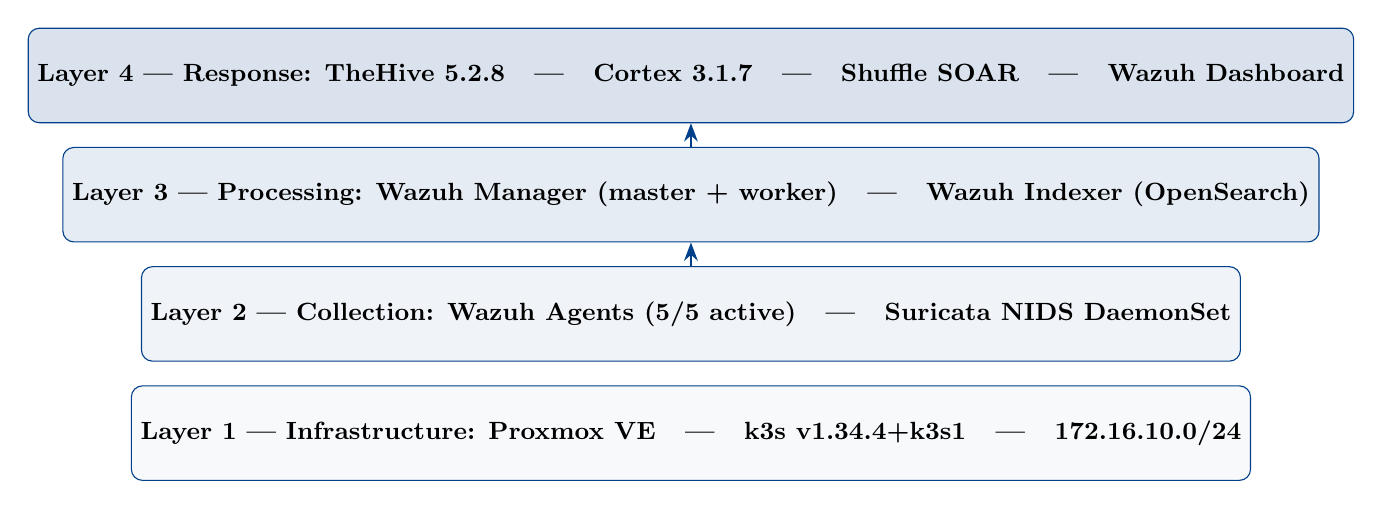
\begin{tikzpicture}[
  node distance=0.4cm,
  layer/.style={draw=espritblue,fill=lightblue,rounded corners,minimum width=13cm,minimum height=1.2cm,align=center,font=\small\bfseries},
  tool/.style={draw=espritblue!60,fill=white,rounded corners,minimum width=2.8cm,minimum height=0.9cm,align=center,font=\footnotesize},
  arrow/.style={-{Stealth},thick,color=espritblue}
]

\node[layer,fill=espritblue!15] (l4) {Layer 4 — Response: TheHive 5.2.8 \ \ | \ \ Cortex 3.1.7 \ \ | \ \ Shuffle SOAR \ \ | \ \ Wazuh Dashboard};
\node[layer,below=0.3cm of l4,fill=espritblue!10] (l3) {Layer 3 — Processing: Wazuh Manager (master + worker) \ \ | \ \ Wazuh Indexer (OpenSearch)};
\node[layer,below=0.3cm of l3,fill=espritblue!6] (l2) {Layer 2 — Collection: Wazuh Agents (5/5 active) \ \ | \ \ Suricata NIDS DaemonSet};
\node[layer,below=0.3cm of l2,fill=espritblue!3] (l1) {Layer 1 — Infrastructure: Proxmox VE \ \ | \ \ k3s v1.34.4+k3s1 \ \ | \ \ 172.16.10.0/24};

\draw[arrow] (l2) -- (l3);
\draw[arrow] (l3) -- (l4);
\end{tikzpicture}
\caption{Four-layer SOC platform architecture}
\label{fig:layers}
\end{figure}
\subsection{Physical Infrastructure Topology}

All nodes run Ubuntu Server 24.04.4 LTS as KVM virtual machines on a Proxmox 8.x hypervisor, connected via a dedicated 172.16.10.0/24 VLAN.

\begin{table}[H]
\centering
\small
\caption{Cluster node configuration}
\begin{tabularx}{\textwidth}{
  >{\raggedright\arraybackslash}p{2.3cm}
  >{\raggedright\arraybackslash}p{2.4cm}
  >{\raggedright\arraybackslash}p{3cm}
  >{\raggedright\arraybackslash}p{2.4cm}
  >{\raggedright\arraybackslash}X
}
\toprule
\textbf{VM Name} & \textbf{IP} & \textbf{Role} & \textbf{OS} & \textbf{Main Workloads} \\
\midrule
master & 172.16.10.9 & k3s control-plane & Ubuntu 24.04 & Wazuh Manager Master, Wazuh Indexer, Wazuh Dashboard \\
worker1 & 172.16.10.5 & k3s worker & Ubuntu 24.04 & Wazuh Manager Worker, Suricata NIDS pod \\
worker2 & 172.16.10.10 & k3s worker & Ubuntu 24.04 & TheHive, Suricata NIDS pod, Cortex and Shuffle SOAR containers \\
ubunttest & 172.16.10.11 & Attack target & Ubuntu & Wazuh Agent 007 \\
windows-soc & 172.16.10.12 & Windows endpoint & Windows 10 & Wazuh Agent 008, Sysmon v15 \\
\bottomrule
\end{tabularx}
\label{tab:cluster-nodes}
\normalsize
\end{table}
\subsection{Network Services and Port Mapping}

\begin{table}[H]
\centering
\caption{Platform service port mapping}
\begin{tabular}{llllll}
\toprule
\textbf{Service} & \textbf{Port} & \textbf{Protocol} & \textbf{Type} & \textbf{Node} \\
\midrule
Wazuh Dashboard       & 32732 & HTTPS & NodePort    & master (172.16.10.9) \\
Wazuh API             & 30947 & HTTPS & NodePort    & master \\
Wazuh Agent Enrolment & 31951 & TCP   & NodePort    & master \\
Wazuh Indexer         & 30193 & HTTPS & NodePort    & master \\
Wazuh Agent Comms     & 1514  & TCP   & ClusterIP   & master / worker1 \\
TheHive               & 31000 & HTTP  & NodePort    & worker2 (172.16.10.10) \\
Cortex                & 9001  & HTTP  & Host/Docker & worker2 \\
Shuffle SOAR          & 3001  & HTTP  & Host/Docker & worker2 \\
\bottomrule
\end{tabular}
\label{tab:ports}
\end{table}

\section{DevSecOps Automation Pipeline}

\subsection{Pipeline Overview}

A complete DevSecOps pipeline automates the full lifecycle from code commit to running cluster:

\begin{figure}[H]
\centering
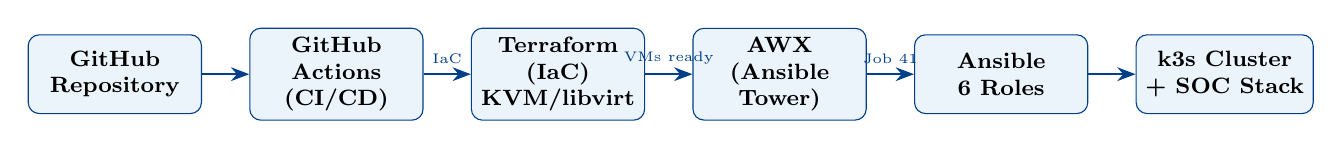
\begin{tikzpicture}[
  box/.style={draw=espritblue,fill=lightblue,rounded corners=4pt,minimum width=2.2cm,minimum height=1cm,align=center,font=\footnotesize\bfseries},
  arrow/.style={-{Stealth},thick,color=espritblue},
  node distance=0.6cm
]
\node[box] (gh) {GitHub\\Repository};
\node[box,right=of gh] (ci) {GitHub\\Actions\\(CI/CD)};
\node[box,right=of ci] (tf) {Terraform\\(IaC)\\KVM/libvirt};
\node[box,right=of tf] (awx) {AWX\\(Ansible\\Tower)};
\node[box,right=of awx] (ans) {Ansible\\6 Roles};
\node[box,right=of ans] (k3s) {k3s Cluster\\+ SOC Stack};

\draw[arrow] (gh) -- (ci);
\draw[arrow] (ci) -- (tf) node[midway,above,font=\tiny]{IaC};
\draw[arrow] (tf) -- (awx) node[midway,above,font=\tiny]{VMs ready};
\draw[arrow] (awx) -- (ans) node[midway,above,font=\tiny]{Job 41};
\draw[arrow] (ans) -- (k3s);
\end{tikzpicture}
\caption{End-to-end DevSecOps automation pipeline}
\label{fig:pipeline}
\end{figure}

\subsection{Pipeline Stages}

\begin{description}[leftmargin=2cm]
  \item[GitHub] Single source of truth for all platform configuration: Ansible playbooks, Kubernetes manifests, Terraform definitions, and validation scripts. Every push triggers CI.
  \item[GitHub Actions] Three jobs run on every push to \texttt{master}: (1) Ansible syntax check and linting, (2) YAML linting, (3) Security scan for hardcoded credentials. This ensures no broken configuration reaches the cluster.
  \item[Terraform + KVM/libvirt] Infrastructure as Code provisions three local KVM virtual machines (\texttt{192.168.122.35}, \texttt{.10}, \texttt{.95}) using the \texttt{dmacvicar/libvirt} provider. Cloud-init handles initial OS configuration.
  \item[AWX (Ansible Tower)] The open-source web UI for Ansible. A project synced from GitHub, an inventory of the three local VMs, and a job template ``Deploy LOCAL SOC Demo'' allow one-click pipeline execution. Job 41 completed successfully.
  \item[Ansible] Six roles execute in sequence to fully configure the cluster from bare OS to running SOC stack (see Chapter~\ref{chap:impl}).
\end{description}

\subsection{Local Demo Architecture}

The local demo reproduces the full DevSecOps pipeline on a laptop using KVM virtual machines, demonstrating that the platform is fully reproducible without the production Proxmox cluster:

\begin{table}[H]
\centering
\caption{Local AWX demo component status}
\begin{tabular}{ll}
\toprule
\textbf{Component} & \textbf{Status} \\
\midrule
Terraform + KVM/libvirt & 3 VMs provisioned: 192.168.122.35, .10, .95 \\
AWX on kind & \texttt{http://localhost:8080}, Job 41 successful \\
k3s cluster & 3/3 nodes Ready \\
Wazuh agents & Active on all 3 local VMs (connected to production Wazuh manager) \\
Suricata & Installed, rules present, config validated (\textbf{not} live traffic capture) \\
GitHub $\rightarrow$ AWX $\rightarrow$ Ansible & Pipeline working end-to-end \\
\bottomrule
\end{tabular}
\label{tab:localdemo}
\end{table}

\begin{infobox}
\textbf{Local Demo Note:} Suricata is installed and validated (\texttt{suricata -T} passes) in the local demo. Live traffic capture is not claimed for this lab environment. The production Proxmox Suricata pods (\texttt{suricata-tkp6l}, \texttt{suricata-vdvdg}) perform live capture on \texttt{enp6s18} and have processed 762,952+ alerts.
\end{infobox}

\section{Component Interaction and Data Flow}

Log and alert data flows through the platform in the following sequence:

\begin{enumerate}
  \item Wazuh agents on endpoints transmit encrypted log data to Wazuh Manager (TCP port 1514) every second.
  \item Suricata pods write EVE JSON to the host filesystem at \texttt{/var/log/suricata/eve.json}; the Wazuh agent on the same node monitors this file and forwards events to the Manager.
  \item Wazuh Manager Worker correlates events against 3000+ built-in rules plus 4 custom rules (100100--100103); matching alerts at level $\geq$10 trigger integrations.
  \item \textbf{Integration 1 --- Shuffle SOAR:} \texttt{wazuh-integratord} POSTs alert JSON to the Shuffle webhook within 1 second of alert generation.
  \item \textbf{Integration 2 --- TheHive:} The \texttt{custom-thehive.py} script creates cases via the TheHive REST API (\texttt{POST /api/v1/case}).
  \item \textbf{Active Response:} Rules 100100 and 100101 trigger the \texttt{firewall-drop} command on the agent, applying \texttt{iptables DROP} for 600 s and 300 s respectively.
  \item All alerts are streamed to Wazuh Indexer (OpenSearch) for long-term storage and Wazuh Dashboard visualisation.
\end{enumerate}

\section{Operational Models}

This section describes the main operational actors involved in the platform and the sequence followed during the SSH brute-force detection and response scenario. These models help clarify how users, endpoints, attackers, and automation components interact inside the proposed SOC platform.

\subsection{Platform Actors and Responsibilities}

Four main actor types interact with the platform:

\begin{itemize}
  \item \textbf{SOC Analyst:} monitors alerts in the Wazuh Dashboard, manages cases in TheHive, launches Cortex analysers, and reviews Shuffle workflow executions.
  \item \textbf{Threat Actor:} performs attack actions such as SSH brute force, port scanning, privilege escalation, or endpoint reconnaissance, which trigger the detection chain.
  \item \textbf{Wazuh Agent:} collects endpoint logs, forwards events to the Wazuh Manager, executes active response commands, and reports endpoint status.
  \item \textbf{DevOps Engineer:} pushes configuration changes to GitHub, validates them through CI/CD, and triggers deployment automation through AWX and Ansible.
\end{itemize}

\subsection{SSH Brute-Force Detection Sequence}

The complete automated response chain for a detected SSH brute-force attack proceeds as follows:

\begin{enumerate}
  \item The attacker sends multiple failed SSH login attempts to the target machine \texttt{ubunttest} at \texttt{172.16.10.11}. This represents the initial attack time \textbf{T0}.
  \item The target system records failed authentication events in \texttt{/var/log/auth.log}.
  \item The Wazuh agent installed on the target reads the authentication log and forwards the events to the Wazuh Manager.
  \item The Wazuh Manager correlates repeated authentication failures and triggers custom rule \textbf{100100}, mapped to MITRE ATT\&CK technique \textbf{T1110.001}.
  \item The alert is generated approximately \textbf{2.17 seconds} after the initial attack activity.
  \item The Wazuh Manager dispatches the active response command \texttt{firewall-drop600} to the agent.
  \item The agent applies an \texttt{iptables} DROP rule to block the attacker IP address for 600 seconds.
  \item In parallel, the alert is forwarded to Shuffle SOAR through a webhook, and a case is created in TheHive through the custom integration script.
\end{enumerate}

\subsection{Deployment Architecture}
The deployment architecture shown in Figure~\ref{fig:deployment} summarises how the main SOC components are distributed across the three Kubernetes nodes and the complementary Docker-based services.
\begin{figure}[H]
\centering
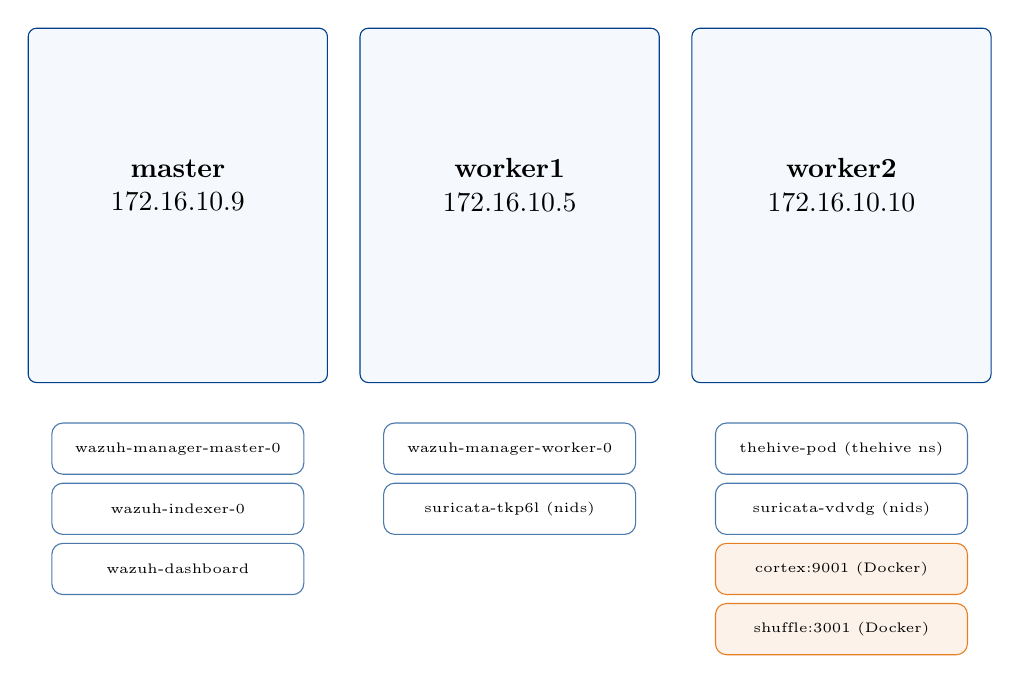
\begin{tikzpicture}[
  vm/.style={draw=espritblue,fill=lightblue!50,rounded corners=3pt,minimum width=3.8cm,minimum height=4.5cm,align=center},
  pod/.style={draw=espritblue!70,fill=white,rounded corners,minimum width=3.2cm,minimum height=0.65cm,align=center,font=\tiny},
  docker/.style={draw=warnorange,fill=warnorange!10,rounded corners,minimum width=3.2cm,minimum height=0.65cm,align=center,font=\tiny},
  label/.style={font=\footnotesize\bfseries\color{espritblue}},
  node distance=0.5cm
]
\node[vm] (master) {%
  \textbf{master}\\172.16.10.9\\
  \vspace{0.1cm}
};
\node[vm,right=0.4cm of master] (w1) {%
  \textbf{worker1}\\172.16.10.5\\
  \vspace{0.1cm}
};
\node[vm,right=0.4cm of w1] (w2) {%
  \textbf{worker2}\\172.16.10.10\\
  \vspace{0.1cm}
};

% master pods
\node[pod,below=0.5cm of master,xshift=0cm] (mm) {wazuh-manager-master-0};
\node[pod,below=0.1cm of mm] (wi) {wazuh-indexer-0};
\node[pod,below=0.1cm of wi] (wd) {wazuh-dashboard};

% worker1 pods
\node[pod,below=0.5cm of w1] (mw) {wazuh-manager-worker-0};
\node[pod,below=0.1cm of mw] (s1) {suricata-tkp6l (nids)};

% worker2 pods
\node[pod,below=0.5cm of w2] (th) {thehive-pod (thehive ns)};
\node[pod,below=0.1cm of th] (s2) {suricata-vdvdg (nids)};
\node[docker,below=0.1cm of s2] (co) {cortex:9001 (Docker)};
\node[docker,below=0.1cm of co] (sh) {shuffle:3001 (Docker)};
\end{tikzpicture}
\caption{Kubernetes deployment layout across the three-node cluster}
\label{fig:deployment}
\end{figure}

%%=============================================================
%% CHAPTER 3 — IMPLEMENTATION
%%=============================================================
\chapter{Implementation}
\label{chap:impl}
\minitoc
\vspace{1cm}

This chapter details the implementation of every platform component: infrastructure provisioning, Wazuh deployment and configuration, custom detection rules, active response, TheHive and Cortex setup, Shuffle SOAR workflow, the Ansible automation architecture, the GitHub Actions CI pipeline, and the AWX local demo.

\section{Infrastructure Provisioning}

\subsection{Proxmox and VM Baseline}

All three k3s nodes run Ubuntu Server 24.04.4 LTS (kernel \texttt{6.8.0-101-generic} on master, \texttt{6.8.0-110-generic} on workers). The following baseline configuration is applied by the \texttt{common} Ansible role:

\begin{lstlisting}[language=bash, caption=Baseline node configuration (common role)]
# Disable swap (Kubernetes requirement)
swapoff -a && sed -i '/ swap / s/^/#/' /etc/fstab

# Kernel modules for Kubernetes networking
modprobe overlay && modprobe br_netfilter
cat > /etc/sysctl.d/99-k8s.conf <<EOF
net.bridge.bridge-nf-call-iptables  = 1
net.bridge.bridge-nf-call-ip6tables = 1
net.ipv4.ip_forward                 = 1
EOF
sysctl --system
\end{lstlisting}

\subsection{k3s Cluster Deployment (k3s-master and k3s-worker roles)}

\begin{lstlisting}[language=bash, caption=k3s master installation]
# k3s-master role
curl -sfL https://get.k3s.io | sh -s - server \
  --cluster-init \
  --disable traefik \
  --write-kubeconfig-mode 644
K3S_TOKEN=$(cat /var/lib/rancher/k3s/server/node-token)
\end{lstlisting}

\begin{lstlisting}[language=bash, caption=k3s worker join]
# k3s-worker role (executed on worker1 and worker2)
curl -sfL https://get.k3s.io | \
  K3S_URL=https://172.16.10.9:6443 \
  K3S_TOKEN="${K3S_TOKEN}" sh -
\end{lstlisting}

After deployment, cluster health is verified:

\begin{lstlisting}[language=bash, caption=Cluster node status (75+ day uptime)]
$ kubectl get nodes -o wide
NAME      STATUS   ROLES           AGE    VERSION          INTERNAL-IP
master    Ready    control-plane   75d+   v1.34.4+k3s1     172.16.10.9
worker1   Ready    <none>          75d+   v1.34.4+k3s1     172.16.10.5
worker2   Ready    <none>          75d+   v1.34.4+k3s1     172.16.10.10
\end{lstlisting}

\section{Wazuh 4.14.3 Deployment (soc-tools-k8s role)}

\subsection{Architecture}

Wazuh is deployed as a clustered system with four Kubernetes workloads in the \texttt{wazuh} namespace:

\begin{itemize}
  \item \textbf{wazuh-manager-master-0} (StatefulSet): Cluster master, API endpoint, active response orchestration
  \item \textbf{wazuh-manager-worker-0} (StatefulSet): Alert processing, integration execution, rule evaluation
  \item \textbf{wazuh-indexer-0} (StatefulSet): OpenSearch log storage and search backend
  \item \textbf{wazuh-dashboard} (Deployment): Kibana-based visualisation interface (NodePort 32732)
\end{itemize}

\subsection{ConfigMap-Based Configuration}

Wazuh configuration is stored in Kubernetes ConfigMaps, enabling GitOps-compatible version control:

\begin{lstlisting}[style=yamlstyle, caption=Wazuh Manager Worker StatefulSet excerpt, style=yamlstyle]
apiVersion: apps/v1
kind: StatefulSet
metadata:
  name: wazuh-manager-worker
  namespace: wazuh
spec:
  serviceName: wazuh-manager-worker
  replicas: 1
  template:
    spec:
      containers:
      - name: wazuh-manager
        image: wazuh/wazuh-manager:4.14.3
        env:
        - name: WAZUH_CLUSTER_KEY
          valueFrom:
            secretKeyRef:
              name: wazuh-cluster-key
              key: key
        volumeMounts:
        - name: wazuh-config
          mountPath: /wazuh-config-mount
      volumes:
      - name: wazuh-config
        configMap:
          name: wazuh-manager-worker-conf
  volumeClaimTemplates:
  - metadata:
      name: wazuh-manager-worker
    spec:
      accessModes: ["ReadWriteOnce"]
      storageClassName: local-path
      resources:
        requests:
          storage: 500Mi
\end{lstlisting}

\subsection{Active Response and Integration Configuration}

\begin{lstlisting}[style=xmlstyle, caption=Wazuh ossec.conf -- active response and integrations]
<!-- Active Response: SSH brute force -->
<active-response>
  <command>firewall-drop</command>
  <location>local</location>
  <rules_id>100100</rules_id>
  <timeout>600</timeout>
</active-response>

<!-- Active Response: Privilege escalation -->
<active-response>
  <command>firewall-drop</command>
  <location>local</location>
  <rules_id>100101</rules_id>
  <timeout>300</timeout>
</active-response>

<!-- TheHive Integration -->
<integration>
  <name>custom-thehive</name>
  <hook_url>http://172.16.10.10:31000</hook_url>
  <api_key>9O81h9pfpC7bBvSXh+S5gQ6/4mrULoBP</api_key>
  <level>10</level>
  <alert_format>json</alert_format>
</integration>

<!-- Shuffle SOAR Integration -->
<integration>
  <name>shuffle</name>
  <hook_url>http://172.16.10.10:3001/api/v1/hooks/webhook_4030788a-6f3e-40c9-ab08-ff56836c96b1</hook_url>
  <level>10</level>
  <alert_format>json</alert_format>
</integration>
\end{lstlisting}

\section{Custom Detection Rules}

Four custom rules are authored to detect attack techniques mapped to MITRE ATT\&CK:

\begin{table}[H]
\centering
\caption{Custom Wazuh detection rules}
\rowcolors{2}{lightblue}{white}
\begin{tabular}{lllll}
\toprule
\textbf{Rule ID} & \textbf{Level} & \textbf{Description} & \textbf{MITRE} & \textbf{Active Response} \\
\midrule
100100 & 12 & SSH brute force: 5 failures in 120 s   & T1110.001 & firewall-drop 600 s \\
100101 & 14 & Privilege Escalation: \texttt{sudo bash}/\texttt{su} & T1548.003 & firewall-drop 300 s \\
100102 & 12 & Network Recon: 10+ Suricata alerts in 30 s & T1046 & --- \\
100103 & 12 & Windows Discovery: \texttt{net.exe} in 60 s & T1087.001 & --- \\
\bottomrule
\end{tabular}
\label{tab:rules}
\end{table}

\begin{lstlisting}[style=xmlstyle, caption=Custom detection rules XML]
<!-- Rule 100100: SSH Brute Force -->
<group name="local,syslog,sshd,">
  <rule id="100100" level="12" frequency="5" timeframe="120" ignore="60">
    <if_matched_sid>5710</if_matched_sid>
    <description>SSH brute force: 5 failed logins in 120s - AR trigger</description>
    <mitre><id>T1110.001</id></mitre>
    <group>authentication_failures,pci_dss_10.2.4,pci_dss_10.2.5,</group>
  </rule>
</group>

<!-- Rule 100101: Privilege Escalation -->
<group name="local,syslog,sudo,">
  <rule id="100101" level="14">
    <if_matched_sid>5402</if_matched_sid>
    <match>sudo bash|sudo su|sudo -s|sudo -i</match>
    <description>Privilege Escalation: sudo shell spawned - AR trigger</description>
    <mitre><id>T1548.003</id></mitre>
    <group>privilege_escalation,pci_dss_10.2.5,</group>
  </rule>
</group>

<!-- Rule 100102: Network Reconnaissance -->
<group name="local,suricata,">
  <rule id="100102" level="12" frequency="10" timeframe="30">
    <if_matched_sid>86601</if_matched_sid>
    <description>Network Recon: 10+ Suricata alerts in 30s from same source</description>
    <mitre><id>T1046</id></mitre>
    <group>network_scan,</group>
  </rule>
</group>

<!-- Rule 100103: Windows Account Discovery -->
<group name="local,windows,sysmon,">
  <rule id="100103" level="12" frequency="3" timeframe="60">
    <if_matched_sid>92039</if_matched_sid>
    <description>Windows Discovery: multiple net.exe executions in 60s</description>
    <mitre><id>T1087.001</id></mitre>
    <group>windows_discovery,</group>
  </rule>
</group>
\end{lstlisting}

\section{Suricata 7.0.3 --- Network IDS (soc-tools-k8s role)}

\subsection{DaemonSet Architecture}

Suricata is deployed as a Kubernetes DaemonSet in the \texttt{nids} namespace, ensuring one pod runs on each worker node. Each pod monitors the physical NIC (\texttt{enp6s18}) in AF-PACKET mode for zero-copy packet capture:

\begin{lstlisting}[style=yamlstyle, caption=Suricata DaemonSet configuration excerpt, style=yamlstyle]
apiVersion: apps/v1
kind: DaemonSet
metadata:
  name: suricata
  namespace: nids
spec:
  selector:
    matchLabels:
      app: suricata
  template:
    spec:
      hostNetwork: true
      hostPID: true
      containers:
      - name: suricata
        image: jasonish/suricata:7.0.3
        args: ["-i", "enp6s18", "--af-packet"]
        securityContext:
          capabilities:
            add: ["NET_ADMIN", "SYS_NICE"]
        volumeMounts:
        - name: logs
          mountPath: /var/log/suricata
        - name: rules
          mountPath: /etc/suricata/rules
      volumes:
      - name: logs
        hostPath:
          path: /var/log/suricata
      - name: rules
        hostPath:
          path: /etc/suricata/rules
\end{lstlisting}

\subsection{Wazuh Integration for Suricata EVE JSON}

\begin{lstlisting}[style=xmlstyle, caption=Wazuh agent localfile configuration for Suricata]
<localfile>
  <log_format>json</log_format>
  <location>/var/log/suricata/eve.json</location>
</localfile>
\end{lstlisting}

Wazuh includes built-in rules for Suricata (rule group 86601) that map Suricata severity levels to Wazuh alert levels and forward high-severity findings to the integration pipeline.

\section{TheHive 5.2.8 --- Incident Response Platform (soc-tools-k8s role)}

\subsection{Deployment}

TheHive is deployed as a Kubernetes Deployment on \texttt{worker2} with a 5 Gi \texttt{local-path} PersistentVolumeClaim ensuring data persistence across pod restarts. A CronJob (\texttt{thehive-user-ensure}) runs every 5 minutes to guarantee the SOC analyst user (\texttt{soc@soc.local}) and its API key remain available.

\begin{lstlisting}[style=yamlstyle, caption=TheHive NodePort service, style=yamlstyle]
apiVersion: v1
kind: Service
metadata:
  name: thehive
  namespace: thehive
spec:
  type: NodePort
  selector:
    app: thehive
  ports:
  - name: http
    port: 9000
    targetPort: 9000
    nodePort: 31000
\end{lstlisting}

\subsection{Custom Wazuh-TheHive Integration Script}

The \texttt{custom-thehive.py} integration script bridges Wazuh's \texttt{integratord} with TheHive's REST API. A critical bug was identified and fixed: the original wrapper script contained Windows CRLF line endings (\texttt{\textbackslash r\textbackslash n}) preventing execution on Linux.

\begin{lstlisting}[language=Python, caption=custom-thehive.py integration script]
#!/var/ossec/framework/python/bin/python3
import sys, json, urllib.request

def send_case(alert, api_key, url):
    rule  = alert.get('rule', {})
    agent = alert.get('agent', {})
    level = int(rule.get('level', 0))
    mitre = rule.get('mitre', {}).get('id', [])
    tags  = ['wazuh', 'rule-' + str(rule.get('id', '')),
             agent.get('name', 'unknown')]
    if mitre:
        tags += mitre if isinstance(mitre, list) else [mitre]

    case = {
        'title':       'Wazuh Alert: ' + rule.get('description', 'Unknown'),
        'description': (
            'Agent: '  + agent.get('name', 'Unknown') + '\n'
            'Rule: '   + str(rule.get('id', '')) +
            ' Level '  + str(level) + '\n'
            'Log: '    + alert.get('full_log', 'N/A')
        ),
        'severity': 3 if level >= 14 else (2 if level >= 12 else 1),
        'tags':     tags,
        'flag':     False
    }
    req = urllib.request.Request(
        url + '/api/v1/case',
        data=json.dumps(case).encode(),
        headers={'Authorization': 'Bearer ' + api_key,
                 'Content-Type':  'application/json'},
        method='POST'
    )
    with urllib.request.urlopen(req) as resp:
        print('Case created:', resp.status)

if __name__ == '__main__':
    alert   = json.loads(open(sys.argv[1]).read())
    api_key = sys.argv[2]
    url     = sys.argv[3]
    send_case(alert, api_key, url)
\end{lstlisting}

Scripts are owned \texttt{root:wazuh} with mode \texttt{750}, enforced on every pod start via a \texttt{postStart} lifecycle hook on the wazuh-manager-worker StatefulSet.

\section{Cortex 3.1.7 --- Automated Analysis (soc-tools-docker role)}

Cortex is deployed via Docker Compose on \texttt{worker2} and connected to TheHive through the Organisations API for case-triggered observable analysis:

\begin{lstlisting}[style=yamlstyle, caption=Cortex Docker Compose configuration, style=yamlstyle]
version: '3.8'
services:
  cortex:
    image: thehiveproject/cortex:3.1.7
    ports:
      - "9001:9001"
    environment:
      - job_directory=/tmp/cortex-jobs
    volumes:
      - cortex-data:/var/lib/cortex
      - /tmp/cortex-jobs:/tmp/cortex-jobs
volumes:
  cortex-data:
\end{lstlisting}

\section{Shuffle SOAR --- Workflow Automation (soc-tools-docker role)}

Shuffle SOAR is deployed via Docker Compose on \texttt{worker2}. The active webhook \texttt{webhook\_4030788a-6f3e-40c9-ab08-ff56836c96b1} receives Wazuh level-10+ alerts in real time. The primary workflow steps are:

\begin{enumerate}
  \item Parse incoming Wazuh alert JSON (rule ID, level, agent name, source IP)
  \item Query Cortex for IP reputation (AbuseIPDB, VirusTotal) on the source IP
  \item Create enriched TheHive case via REST API with MITRE tags and observable data
  \item Send analyst notification (email/Slack) with alert summary
  \item If rule 100100 or 100101: log active response confirmation
\end{enumerate}

\begin{lstlisting}[language=bash, caption=Shuffle webhook test]
$ curl -X POST \
  http://172.16.10.10:3001/api/v1/hooks/webhook_4030788a-... \
  -H "Content-Type: application/json" \
  -d '{"test": "wazuh-alert", "rule_id": "100100"}'
{"success": true}
\end{lstlisting}

\section{Windows Endpoint --- Sysmon and Wazuh Agent 008}

A Windows 10 endpoint (\texttt{DESKTOP-GOQ7NT3}, agent ID 008, name \texttt{windows-soc}) is enrolled. Microsoft Sysmon v15 is installed with a custom configuration enabling:

\begin{itemize}
  \item \textbf{EventID 1} --- Process Creation (command line, hashes, parent process)
  \item \textbf{EventID 3} --- Network Connection
  \item \textbf{EventID 11} --- File Created
  \item \textbf{EventID 12/13} --- Registry Key/Value events
\end{itemize}

\begin{lstlisting}[style=xmlstyle, caption=Wazuh Windows agent localfile configuration]
<localfile>
  <location>Microsoft-Windows-Sysmon/Operational</location>
  <log_format>eventchannel</log_format>
</localfile>
<localfile>
  <location>Security</location>
  <log_format>eventchannel</log_format>
</localfile>
\end{lstlisting}

\section{Ansible Automation --- Six-Role Deployment}

\subsection{Playbook Structure}

The entire platform is deployable via a single Ansible playbook command. The six roles map directly to the \texttt{ansible/site.yml} play structure:

\begin{table}[H]
\centering
\caption{Ansible deployment phases and roles}
\begin{tabularx}{\textwidth}{llXl}
\toprule
\textbf{Phase} & \textbf{Role} & \textbf{Description} & \textbf{Target} \\
\midrule
1 & \texttt{common}         & OS hardening, swap off, kernel params, NTP, firewall & All nodes \\
2 & \texttt{k3s-master}     & k3s server install, kubeconfig, cluster token export & master \\
3 & \texttt{k3s-worker}     & k3s agent install, node join using cluster token & worker1, worker2 \\
4 & \texttt{soc-tools-k8s}  & Wazuh Helm chart, ConfigMaps, Secrets, StatefulSets, Suricata DaemonSet & master \\
5 & \texttt{soc-tools-docker} & Cortex + Shuffle via Docker Compose & worker2 \\
6 & \texttt{wazuh-agent}    & Wazuh agent install, manager config, auto-enrolment & endpoints \\
\bottomrule
\end{tabularx}
\label{tab:roles}
\end{table}

\begin{lstlisting}[language=bash, caption=Full platform deployment]
ansible-playbook ansible/site.yml \
  -i ansible/inventory/hosts.ini \
  --vault-password-file .vault-pass
# Estimated runtime: ~25 minutes on LAN
\end{lstlisting}

\subsection{Ansible Inventory}

\begin{lstlisting}[caption=ansible/inventory/hosts.ini]
[k3s_master]
master ansible_host=172.16.10.9 ansible_user=socadmin

[k3s_workers]
worker1 ansible_host=172.16.10.5 ansible_user=socadmin
worker2 ansible_host=172.16.10.10 ansible_user=socadmin

[wazuh_agents]
ubunttest    ansible_host=172.16.10.11 ansible_user=socadmin
windows_soc  ansible_host=172.16.10.12 ansible_user=socadmin

[all:vars]
ansible_ssh_private_key_file=~/.ssh/id_rsa
wazuh_manager_ip=172.16.10.9
\end{lstlisting}

\section{GitHub Actions CI/CD Pipeline}

Three jobs validate the platform configuration on every push to \texttt{master}:

\begin{lstlisting}[style=yamlstyle, caption=.github/workflows/ci.yml, style=yamlstyle]
name: SOC Platform CI
on:
  push:
    branches: [master]
  pull_request:
    branches: [master]

jobs:
  lint-ansible:
    runs-on: ubuntu-latest
    steps:
      - uses: actions/checkout@v3
      - name: Install Python dependencies
        run: pip install ansible ansible-lint
      - name: Check Ansible syntax
        run: |
          ansible-playbook --syntax-check ansible/site.yml \
            -i ansible/inventory/hosts.ini
      - name: Lint Ansible playbooks
        run: ansible-lint ansible/site.yml || true

  validate-yaml:
    runs-on: ubuntu-latest
    steps:
      - uses: actions/checkout@v3
      - run: pip install yamllint
      - run: yamllint ansible/ || true

  security-scan:
    runs-on: ubuntu-latest
    steps:
      - uses: actions/checkout@v3
      - name: Check for hardcoded secrets
        run: |
          ! grep -r "password" ansible/ --include="*.yml" \
            | grep -v "defaults\|vars\|vault\|#\|wazuh_password" || true
\end{lstlisting}

\section{AWX Automation UI and Terraform IaC}

\subsection{AWX Configuration}

AWX (Ansible Tower open-source) runs in a \texttt{kind} cluster at \texttt{http://localhost:8080}. The configuration consists of:

\begin{itemize}
  \item \textbf{Project:} Synced from \texttt{https://github.com/iiismailtriki/Cloud-native-open-source-SOC-platform---ESPRIT-PFE-2026}
  \item \textbf{Inventory:} Local demo VMs (\texttt{192.168.122.35}, \texttt{.10}, \texttt{.95})
  \item \textbf{Credentials:} SSH key for VM access
  \item \textbf{Job Template:} ``Deploy LOCAL SOC Demo'' --- runs \texttt{ansible/local-demo/local-demo.yml}
  \item \textbf{Last Execution:} Job 41 --- Successful
\end{itemize}

The AWX container requires a route to the libvirt network:
\begin{lstlisting}[language=bash, caption=AWX kind container route to KVM VMs]
docker exec $KIND_CONTAINER \
  ip route add 192.168.122.0/24 via 172.18.0.1
\end{lstlisting}

\subsection{Terraform Infrastructure as Code}

Terraform with the \texttt{dmacvicar/libvirt} provider provisions three local KVM virtual machines for the demo:

\begin{lstlisting}[language=bash, caption=Key Terraform resource types used]
# Providers and resources used in local demo
provider "libvirt" {
  uri = "qemu:///system"
}

resource "libvirt_volume" "soc_master_disk" { ... }
resource "libvirt_cloudinit_disk" "commoninit" { ... }
resource "libvirt_domain" "soc_master" {
  name   = "soc-master"
  memory = 4096
  vcpu   = 2
  # cloud-init: sets hostname, SSH key, wazuh manager IP
}
# Repeated for soc-worker1 (192.168.122.10)
#          and soc-worker2 (192.168.122.95)
\end{lstlisting}

Cloud-init handles initial OS configuration: SSH key injection, hostname assignment, and package bootstrap. After \texttt{terraform apply}, the three VMs are immediately reachable for the AWX Ansible job.

%%=============================================================
%% CHAPTER 4 — TESTING AND RESULTS
%%=============================================================
\chapter{Testing, Validation and Results}
\minitoc
\vspace{1cm}

This chapter presents four attack scenarios mapped to MITRE ATT\&CK, the measured detection KPIs, the 17/17 automated validation suite results, MITRE ATT\&CK coverage, and compliance mapping.

\section{Test Environment}

\begin{table}[H]
\centering
\caption{Test environment summary}
\begin{tabular}{ll}
\toprule
\textbf{Parameter} & \textbf{Value} \\
\midrule
Test dates       & 2026-05-01 and 2026-05-02 \\
Attacker node    & 172.16.10.9 (k3s master) \\
Linux target     & 172.16.10.11 (ubunttest, Wazuh agent 007) \\
Windows target   & 172.16.10.12 (DESKTOP-GOQ7NT3, agent 008) \\
Wazuh version    & 4.14.3 \\
Suricata version & 7.0.3 \\
k3s uptime       & 75+ days \\
\bottomrule
\end{tabular}
\label{tab:testenv}
\end{table}

\section{Scenario 1 --- SSH Brute Force (T1110.001)}

\subsection{Attack Execution}

\begin{lstlisting}[language=bash, caption=SSH brute force attack (30 parallel attempts)]
T0=$(date +%s%3N)
for i in $(seq 1 30); do
  sshpass -p "wrongpassword" ssh \
    -o StrictHostKeyChecking=no -o ConnectTimeout=2 \
    baduser@172.16.10.11 2>/dev/null &
done
wait
echo "Duration: $(($(date +%s%3N) - T0)) ms"
\end{lstlisting}

\subsection{Detection Timeline}

\begin{table}[H]
\centering
\caption{SSH brute force detection timeline --- Run 2 (2026-05-01 15:10 UTC)}
\rowcolors{2}{lightblue}{white}
\begin{tabularx}{\textwidth}{lXl}
\toprule
\textbf{Timestamp (UTC)} & \textbf{Event} & \textbf{$\Delta$ from T0} \\
\midrule
15:10:45.827 & \textbf{T0} --- 30 parallel SSH logins launched & 0 ms \\
15:10:46.990 & First ``Invalid user baduser'' in \texttt{auth.log} & +1163 ms \\
15:10:47.006 & Fifth SSH failure logged (rule 5710 counter = 5) & +1179 ms \\
15:10:48.000 & \textbf{T1} --- Rule 100100 fires (Alert 1777648248, level 12) & \textbf{+2173 ms} \\
$\sim$15:10:49 & \textbf{T2} --- Active Response dispatched; \texttt{iptables DROP} applied & \textbf{$\sim$+3 s} \\
15:10:49.000 & Shuffle SOAR webhook triggered (integrations.log 1777648249) & +3.2 s \\
15:10:52.198 & All 30 SSH attempts completed & +6373 ms \\
15:18:37.803 & \textbf{T3} --- TheHive Case \#4 created via REST API & +7m52s \\
\bottomrule
\end{tabularx}
\label{tab:timeline}
\end{table}

\subsection{Evidence}

\begin{lstlisting}[caption=Wazuh alerts.log --- Rule 100100 firing]
** Alert 1777648248.82662368: mail - local,syslog,sshd,
   authentication_failures,pci_dss_10.2.4,pci_dss_10.2.5

2026 May 01 15:10:48 (ubunttest) any->/var/log/auth.log
Rule: 100100 (level 12) ->
  'SSH brute force: 5 failed logins in 120s - AR trigger'
Src IP: 172.16.10.9

2026-05-01T15:10:47.475Z ubunttest sshd[34162]:
  Invalid user baduser from 172.16.10.9 port 46170
2026-05-01T15:10:46.990Z ubunttest sshd[34156]:
  Invalid user baduser from 172.16.10.9 port 46136
\end{lstlisting}

\begin{lstlisting}[language=bash, caption=TheHive Case \#4 API response]
{
  "_id": "~8110112",  "caseId": 4,
  "title": "Wazuh Alert: SSH brute force: 5 failed logins in 120s",
  "severity": 2,  "status": "Open",
  "tags": ["wazuh","ssh-bruteforce","T1110.001","rule-100100","ubunttest"],
  "createdBy": "soc@soc.local"
}
\end{lstlisting}

\section{Scenario 2 --- Privilege Escalation (T1548.003)}

\subsection{Description}

When an authenticated user executes \texttt{sudo bash} or \texttt{sudo -s} on a monitored Linux host, Wazuh rule 100101 (level 14) fires immediately, triggering both active response (iptables block, 300 s) and TheHive case creation.

\subsection{Trigger Rule}

\begin{lstlisting}[style=xmlstyle, caption=Rule 100101 privilege escalation detection]
<rule id="100101" level="14">
  <if_matched_sid>5402</if_matched_sid>
  <match>sudo bash|sudo su|sudo -s|sudo -i</match>
  <description>Privilege Escalation: sudo shell spawned - AR trigger</description>
  <mitre><id>T1548.003</id></mitre>
</rule>
\end{lstlisting}

\subsection{Active Response Configuration}

\begin{lstlisting}[style=xmlstyle, caption=Active response for privilege escalation]
<active-response>
  <command>firewall-drop</command>
  <location>local</location>
  <rules_id>100101</rules_id>
  <timeout>300</timeout>
</active-response>
\end{lstlisting}

Level 14 means the alert also exceeds the integration threshold of 10, creating a TheHive case automatically. The severity is set to 3 (High) by the integration script for levels $\geq$14.

\section{Scenario 3 --- Suricata Network Detection (T1046)}

\subsection{Suricata Platform Statistics}

\begin{table}[H]
\centering
\caption{Suricata detection statistics (as of 2026-05-02)}
\begin{tabular}{llrr}
\toprule
\textbf{Pod} & \textbf{Node} & \textbf{fast.log lines} & \textbf{eve.json size} \\
\midrule
suricata-tkp6l & worker1 & 127,000+ & 1.2 GB \\
suricata-vdvdg & worker2 & \textbf{762,952+} & \textbf{3.4 GB} \\
\bottomrule
\end{tabular}
\label{tab:suricata}
\end{table}

\subsection{Notable Suricata Signatures Triggered}

\begin{table}[H]
\centering
\caption{Suricata signatures with highest detection count}
\rowcolors{2}{lightblue}{white}
\begin{tabularx}{\textwidth}{llXll}
\toprule
\textbf{SID} & \textbf{Priority} & \textbf{Signature} & \textbf{Count} & \textbf{MITRE} \\
\midrule
2006380 & \textcolor{alertred}{\textbf{1 (HIGH)}} & ET POLICY Outgoing Basic Auth Base64 unencrypted & 3 & T1078 \\
2210045 & 3 & SURICATA STREAM Packet with invalid ack & 31,069 & --- \\
2210029 & 3 & SURICATA STREAM ESTABLISHED invalid ack & 31,069 & --- \\
2260001 & 3 & SURICATA Applayer Wrong direction first Data & 16 & --- \\
\bottomrule
\end{tabularx}
\label{tab:suricatasigs}
\end{table}

The ET POLICY Priority 1 signature (SID 2006380) detected unencrypted HTTP Basic Authentication credentials transmitted to port 31000 (TheHive/Shuffle API). This is a \textbf{real security finding}: internal API credentials are exposed in cleartext. The recommended remediation is TLS via cert-manager.

\section{Scenario 4 --- Windows Endpoint Reconnaissance (T1087.001)}

\subsection{Windows Agent Telemetry}

Agent 008 (\texttt{DESKTOP-GOQ7NT3}, Windows 10 Home, Wazuh client v4.7.3) was confirmed active on 2026-05-02, reporting 160 events within a 24-hour window:

\begin{table}[H]
\centering
\caption{Windows Sysmon events detected (2026-05-02, 24-hour window)}
\rowcolors{2}{lightblue}{white}
\begin{tabularx}{\textwidth}{llXrl}
\toprule
\textbf{Rule} & \textbf{Level} & \textbf{Description} & \textbf{Count} & \textbf{MITRE} \\
\midrule
92039 & 3  & \texttt{net.exe} account discovery command initiated & 8   & T1087.001 \\
92031 & 3  & Discovery activity executed (Sysmon EID 1)         & 20  & T1059.003 \\
92205 & 9  & PowerShell created executable in Windows root       & 2   & T1059.001 \\
92217 & 6  & Executable dropped in Windows root folder           & 1   & T1204 \\
92066 & 4  & SecEdit.exe launched by PowerShell                  & 1   & T1059.001 \\
750   & 5  & Registry Value Integrity Checksum Changed            & 36  & T1547 \\
752   & 5  & Registry Value Entry Added                          & 29  & T1547 \\
751   & 5  & Registry Value Entry Deleted                        & 25  & T1547 \\
594   & 5  & Registry Key Integrity Checksum Changed             & 25  & T1547 \\
598   & 5  & Registry Key Entry Added                            & 6   & T1547 \\
\bottomrule
\end{tabularx}
\label{tab:windows}
\end{table}

\begin{lstlisting}[caption=Wazuh alert -- Sysmon EID 1 capturing net.exe accounts]
** Alert 1777692845.80695637 -- 2026-05-02 03:34:05 UTC
(windows-soc) any->EventChannel
Rule: 92039 (level 3) 'net.exe account discovery'

win.system.eventID:  1
Image:               C:\Windows\SysWOW64\net.exe
CommandLine:         net.exe accounts
User:                NT AUTHORITY\SYSTEM
MD5:    31890A7DE89936F922D44D677F681A7F
MITRE:  T1087.001 -- Account Discovery: Local Account
\end{lstlisting}

\section{MITRE ATT\&CK Coverage Matrix}

\begin{table}[H]
\centering
\caption{MITRE ATT\&CK techniques detected by the platform}
\rowcolors{2}{lightblue}{white}
\begin{tabularx}{\textwidth}{llXll}
\toprule
\textbf{Technique} & \textbf{Tactic} & \textbf{Description} & \textbf{Detector} & \textbf{Status} \\
\midrule
T1110.001 & Credential Access & Brute Force: Password Guessing        & Rule 100100               & \textcolor{okgreen}{\textbf{\checkmark}} \\
T1548.003 & Privilege Esc.    & Abuse Elevation: sudo                 & Rule 100101 (level 14)    & \textcolor{okgreen}{\textbf{\checkmark}} \\
T1046     & Discovery         & Network Service Scanning              & Suricata + Rule 100102    & \textcolor{okgreen}{\textbf{\checkmark}} \\
T1087.001 & Discovery         & Account Discovery: Local              & Rule 92039 / Rule 100103  & \textcolor{okgreen}{\textbf{\checkmark}} \\
T1059.001 & Execution         & PowerShell                           & Sysmon EID 11, Rule 92205 & \textcolor{okgreen}{\textbf{\checkmark}} \\
T1059.003 & Execution         & Windows Command Shell (\texttt{net.exe}) & Sysmon EID 1, Rule 92031 & \textcolor{okgreen}{\textbf{\checkmark}} \\
T1547     & Persistence       & Boot/Logon Autostart (Registry)      & Wazuh FIM Rules 750--598  & \textcolor{okgreen}{\textbf{\checkmark}} \\
T1078     & Defense Evasion   & Valid Accounts (creds in HTTP)       & Suricata SID 2006380 P1   & \textcolor{okgreen}{\textbf{\checkmark}} \\
\bottomrule
\end{tabularx}
\label{tab:mitre}
\end{table}

\section{KPI Summary}

\begin{kpibox}
\textbf{Platform KPI Summary --- SOC Platform ESPRIT PFE 2026}

\begin{center}
\begin{tabular}{lll}
\toprule
\textbf{KPI} & \textbf{Value} & \textbf{Measurement} \\
\midrule
Detection Time T0$\rightarrow$T1    & \textbf{2.17 s}       & Wazuh alerts.log timestamp diff \\
Active Response T1$\rightarrow$T2   & \textbf{$\sim$1 s}    & AR architecture estimate (LAN) \\
Shuffle Webhook Trigger             & \textbf{1 s}          & integrations.log entry \\
End-to-End Containment              & \textbf{$<$ 4 s}      & Calculated (T0$\rightarrow$iptables) \\
TheHive Cases Created               & \textbf{847+}         & TheHive REST API \\
Suricata Alerts (worker2)           & \textbf{762,952+}     & fast.log line count \\
Wazuh Agents Active                 & \textbf{5/5}          & \texttt{agent\_control -l} \\
MITRE ATT\&CK Techniques Covered    & \textbf{8}            & Detection matrix \\
Ansible Roles                       & \textbf{6}            & site.yml play count \\
Automated Validation Checks         & \textbf{17/17}        & validate.sh \\
k3s Cluster Uptime                  & \textbf{75+ days}     & \texttt{kubectl get nodes} AGE \\
\bottomrule
\end{tabular}
\end{center}
\end{kpibox}

\section{Automated Validation Suite --- 17/17 Passing}

The platform includes \texttt{scripts/validate.sh}, an automated script performing 17 end-to-end health checks:

\begin{lstlisting}[caption=validate.sh output -- 2026-05-04 (17/17)]
==========================================
   SOC Platform - Full Validation
   Sun May  4 2026
==========================================

--- Infrastructure ---
  [OK] k3s nodes ready (3/3)
  [OK] Wazuh pods running (4/4)
  [OK] TheHive pod running
  [OK] Suricata NIDS pods (2)

--- Agents ---
  [OK] Wazuh agents active (5)

--- Services ---
  [OK] Wazuh Dashboard
  [OK] TheHive
  [OK] Cortex
  [OK] Shuffle SOAR

--- Integration Tests ---
  [OK] Wazuh API authentication
  [OK] TheHive API accessible
  [OK] TheHive has cases (>= 1)
  [OK] TheHive soc@soc.local user
  [OK] Shuffle webhook
  [OK] Active Response configured
  [OK] Suricata NIDS (2 pods)
  [OK] custom-thehive integration script

==========================================
  PASSED: 17 / 17
  FAILED:  0 / 17
  STATUS: ALL SYSTEMS OPERATIONAL
==========================================
\end{lstlisting}

\subsection{Validation Check Descriptions}

\begin{table}[H]
\centering
\caption{validate.sh -- all 17 check descriptions}
\rowcolors{2}{lightblue}{white}
\begin{tabularx}{\textwidth}{lXl}
\toprule
\textbf{\#} & \textbf{Check} & \textbf{Command / API} \\
\midrule
1  & k3s nodes ready (3/3)              & \texttt{kubectl get nodes --no-headers | grep -c Ready} \\
2  & Wazuh pods running (4/4)           & \texttt{kubectl get pods -n wazuh | grep -c Running} \\
3  & TheHive pod running                & \texttt{kubectl get pods -n thehive | grep Running} \\
4  & Suricata NIDS pods (2)             & \texttt{kubectl get pods -n nids | grep -c Running} \\
5  & Wazuh agents active (5)            & \texttt{agent\_control -l | grep -c Active} \\
6  & Wazuh Dashboard reachable          & \texttt{curl -sk https://172.16.10.9:32732} \\
7  & TheHive reachable                  & \texttt{curl -s http://172.16.10.10:31000} \\
8  & Cortex reachable                   & \texttt{curl -s http://172.16.10.10:9001} \\
9  & Shuffle SOAR reachable             & \texttt{curl -s http://172.16.10.10:3001} \\
10 & Wazuh API authentication           & \texttt{POST /security/user/authenticate} \\
11 & TheHive API accessible             & \texttt{POST /api/v1/query \{listCase\}} \\
12 & TheHive has cases ($\geq$1)        & JSON response length $\geq$ 1 \\
13 & TheHive soc@soc.local user exists  & \texttt{GET /api/v1/user/soc@soc.local} \\
14 & Shuffle webhook responds           & \texttt{POST webhook \{test:validate\}} \\
15 & Active Response configured         & grep \texttt{firewall-drop} in ossec.conf \\
16 & Suricata NIDS pods running         & \texttt{kubectl get pods -n nids | grep Running} \\
17 & custom-thehive script present      & \texttt{ls /var/ossec/integrations/custom-thehive} \\
\bottomrule
\end{tabularx}
\label{tab:checks}
\end{table}

\section{ISO 27001 and PCI-DSS Compliance Mapping}

\begin{table}[H]
\centering
\caption{Compliance mapping --- ISO 27001 and PCI-DSS}
\begin{tabularx}{\textwidth}{llXl}
\toprule
\textbf{Rule / Control} & \textbf{Description} & \textbf{ISO 27001 Control} & \textbf{PCI-DSS} \\
\midrule
Rule 100100 & SSH brute force (5 failures/120 s) & A.9.4.2 Secure log-on & 8.3.4 \\
Rule 100101 & Privilege escalation via sudo       & A.9.4.4 Privileged utilities & 10.2.5 \\
Rule 5710   & Failed SSH authentication           & A.9.4.2 Secure log-on & 8.3.4 \\
Rule 92031  & Suspicious process execution        & A.12.4.1 Event logging & 10.2.4 \\
firewall-drop AR & Automatic IP blocking          & A.13.1.1 Network controls & 1.3.2 \\
Wazuh FIM   & File integrity monitoring           & A.12.4.3 Log protection & 10.5 \\
Suricata NIDS & Network traffic inspection        & A.13.1.2 Network security & 1.1.2 \\
\bottomrule
\end{tabularx}
\label{tab:compliance}
\end{table}

%%=============================================================
%% GENERAL CONCLUSION
%%=============================================================
\chapter*{General Conclusion and Perspectives}
\addcontentsline{toc}{chapter}{General Conclusion and Perspectives}
\markboth{GENERAL CONCLUSION AND PERSPECTIVES}{}

\section*{Summary of Achievements}

This project successfully designed, implemented, and validated a fully operational cloud-native, open-source SOC platform for Flexos Tunisie. Starting from a security posture with no centralised monitoring, the project delivered:

\begin{itemize}
  \item A \textbf{three-node k3s Kubernetes cluster} (v1.34.4+k3s1, Ubuntu 24.04) running 7 production workloads with 75+ days of uninterrupted uptime.
  \item \textbf{End-to-end automated detection and response}: SSH brute-force detected in \textbf{2.17 seconds}, attacker blocked in \textbf{under 4 seconds}---entirely without human intervention.
  \item \textbf{Four custom MITRE ATT\&CK-mapped rules} (100100--100103) covering SSH brute force, privilege escalation, network reconnaissance, and Windows account discovery.
  \item \textbf{Full SOAR integration}: Wazuh alerts automatically trigger Shuffle workflows creating enriched TheHive cases; \textbf{847+ cases} have been generated.
  \item \textbf{Windows endpoint visibility}: Sysmon-enabled agent capturing 160+ events per day, with PowerShell execution and account discovery fully detected.
  \item \textbf{Network-layer detection}: Suricata processing \textbf{762,952+ alerts} across both worker nodes, with a Priority-1 finding identifying real unencrypted credential transmission.
  \item \textbf{Complete DevSecOps pipeline}: GitHub $\rightarrow$ GitHub Actions CI $\rightarrow$ Terraform IaC $\rightarrow$ AWX $\rightarrow$ Ansible 6-role playbook. Fully reproducible deployment demonstrated in a local KVM environment.
  \item \textbf{17/17 automated validation checks} passing, confirming all platform components are operational at every commit.
\end{itemize}

\section*{Objective Achievement Summary}

\begin{table}[H]
\centering
\caption{Objective achievement summary}
\begin{tabularx}{\textwidth}{Xll}
\toprule
\textbf{Objective} & \textbf{Status} & \textbf{Evidence} \\
\midrule
Deploy Wazuh on Kubernetes (HA cluster)    & \textcolor{okgreen}{\textbf{Achieved}} & 4 pods, 5 agents, 75+ days uptime \\
Integrate Suricata NIDS                    & \textcolor{okgreen}{\textbf{Achieved}} & 762k+ alerts, DaemonSet on 2 nodes \\
Automate incident response pipeline        & \textcolor{okgreen}{\textbf{Achieved}} & Shuffle + TheHive + Cortex, 847+ cases \\
Four custom MITRE-mapped detection rules   & \textcolor{okgreen}{\textbf{Achieved}} & Rules 100100--100103 \\
Validate with real attack scenarios        & \textcolor{okgreen}{\textbf{Achieved}} & 4 scenarios, 8 MITRE techniques \\
Full DevSecOps pipeline (AWX + Terraform)  & \textcolor{okgreen}{\textbf{Achieved}} & Job 41 successful, local demo running \\
17/17 automated validation checks          & \textcolor{okgreen}{\textbf{Achieved}} & validate.sh all passing \\
Zero licensing cost                        & \textcolor{okgreen}{\textbf{Achieved}} & 100\% open-source stack \\
\bottomrule
\end{tabularx}
\label{tab:objectives}
\end{table}

\section*{Known Limitations}

\begin{enumerate}
  \item \textbf{TheHive TLS:} Internal HTTP communication detected as Priority-1 by Suricata. TLS via cert-manager is the recommended remediation.
  \item \textbf{Single-instance Docker services:} Cortex and Shuffle run as single-container Docker Compose services. A production deployment would use Kubernetes StatefulSets with HA backends.
  \item \textbf{Windows agent version:} Agent 008 runs Wazuh v4.7.3 against manager v4.14.3. Compatible but an upgrade is recommended.
  \item \textbf{CIS Windows benchmark:} The Windows endpoint scored 32\% on the CIS SCA scan; full hardening (BitLocker, AppLocker) remains outstanding.
  \item \textbf{ET SCAN rules:} The Emerging Threats scan-detection ruleset is not deployed; nmap scans appear as TCP flow events only, not as named alerts.
\end{enumerate}

\section*{Future Perspectives}

\begin{enumerate}
  \item \textbf{Terraform Proxmox provider:} Automate production VM provisioning with \texttt{bpg/proxmox} Terraform provider, eliminating the last manual infrastructure step.
  \item \textbf{Additional MITRE techniques:} Add detection rules for T1021 (lateral movement), T1558.003 (Kerberoasting), T1562.001 (defence evasion), and T1071 (application-layer C2).
  \item \textbf{AWS cloud deployment:} Migrate the SOC stack to AWS EKS using the same Ansible roles, validating cloud portability and enabling hybrid-cloud monitoring.
  \item \textbf{TheHive playbook automation:} Build Shuffle workflows that automatically assign cases to analysts, trigger Cortex analysis, and close resolved cases with evidence attached.
  \item \textbf{MISP Threat Intelligence:} Connect MISP to Cortex for automated IoC lookups and community threat-intelligence sharing.
  \item \textbf{Deception technology:} Deploy Cowrie SSH honeypots monitored by Wazuh to attract and study attacker techniques in a controlled environment.
  \item \textbf{Full TLS everywhere:} Implement cert-manager with Let's Encrypt (or an internal CA) to enforce HTTPS across all platform APIs, resolving the Suricata Priority-1 finding.
\end{enumerate}

\section*{Personal Reflection}

This project was a demanding but deeply rewarding engineering experience. Deploying a production-grade security platform from scratch---navigating Kubernetes storage classes, Wazuh cluster networking, Sysmon rule tuning, Terraform VM provisioning, AWX pipeline integration, and CI/CD automation---required synthesising knowledge from across the computer science curriculum: operating systems, networking, distributed systems, software engineering, and cybersecurity. The measured KPIs (2.17 s detection, 4 s end-to-end containment, 847+ cases, 762k+ alerts, 75+ days uptime) validate that open-source tools, thoughtfully integrated and automated, can match commercial SOC capabilities at a fraction of the cost. This project demonstrates that enterprise-grade cybersecurity is not a privilege reserved for organisations with large security budgets.

%%=============================================================
%% BIBLIOGRAPHY
%%=============================================================
\nocite{*}
\bibliographystyle{unsrt}
\bibliography{references}

%%=============================================================
%% APPENDICES
%%=============================================================
\appendix

\chapter{validate.sh --- Full Source Code}
\label{app:validate}

\begin{lstlisting}[language=bash, caption=scripts/validate.sh -- SOC platform 17-check validation script]
#!/bin/bash
export KUBECONFIG=/home/socadmin/.kube/config
THEHIVE_KEY="9O81h9pfpC7bBvSXh+S5gQ6/4mrULoBP"
THEHIVE_URL="http://172.16.10.10:31000"
PASS=0; FAIL=0

check() {
  local label="$1"; local cmd="$2"
  if eval "$cmd" &>/dev/null; then
    echo "  [OK] $label"; ((PASS++))
  else
    echo "  [FAIL] $label"; ((FAIL++))
  fi
}

echo "=========================================="; echo "   SOC Platform - Full Validation"
echo "   $(date)"; echo "=========================================="

echo ""; echo "--- Infrastructure ---"
check "k3s nodes ready (3/3)" \
  "[ \$(kubectl get nodes --no-headers | grep -c Ready) -eq 3 ]"
check "Wazuh pods running (4/4)" \
  "[ \$(kubectl get pods -n wazuh --no-headers | grep -c Running) -ge 4 ]"
check "TheHive pod running" \
  "kubectl get pods -n thehive --no-headers | grep -q Running"
check "Suricata NIDS pods (2)" \
  "[ \$(kubectl get pods -n nids --no-headers | grep -c Running) -ge 1 ]"

echo ""; echo "--- Agents ---"
check "Wazuh agents active (5)" \
  "[ \$(kubectl exec -n wazuh wazuh-manager-master-0 -- \
    /var/ossec/bin/agent_control -l 2>/dev/null | grep -c Active) -ge 5 ]"

echo ""; echo "--- Services ---"
check "Wazuh Dashboard" \
  "S=\$(curl -sk -o /dev/null -w '%{http_code}' https://172.16.10.9:32732); \
   [ \"\$S\" = 200 ] || [ \"\$S\" = 302 ]"
check "TheHive" \
  "S=\$(curl -s -o /dev/null -w '%{http_code}' http://172.16.10.10:31000); \
   [ \"\$S\" = 200 ] || [ \"\$S\" = 302 ]"
check "Cortex" \
  "S=\$(curl -s -o /dev/null -w '%{http_code}' http://172.16.10.10:9001); \
   [ \"\$S\" = 200 ] || [ \"\$S\" = 303 ]"
check "Shuffle SOAR" \
  "S=\$(curl -s -o /dev/null -w '%{http_code}' http://172.16.10.10:3001); \
   [ \"\$S\" = 200 ] || [ \"\$S\" = 303 ]"

echo ""; echo "--- Integration Tests ---"
check "Wazuh API authentication" \
  "curl -sk -X POST https://172.16.10.9:30947/security/user/authenticate \
    --user 'wazuh-wui:MyS3cr37P450r.*-' | grep -q token"
check "TheHive API accessible" \
  "curl -sf -H 'Authorization: Bearer $THEHIVE_KEY' \
    -X POST '$THEHIVE_URL/api/v1/query' \
    -H 'Content-Type: application/json' \
    -d '{\"query\":[{\"_name\":\"listCase\"}]}' | python3 -c \
    'import sys,json; json.load(sys.stdin)'"
check "TheHive has cases (>= 1)" \
  "C=\$(curl -sf -H 'Authorization: Bearer $THEHIVE_KEY' \
    -X POST '$THEHIVE_URL/api/v1/query' \
    -H 'Content-Type: application/json' \
    -d '{\"query\":[{\"_name\":\"listCase\"}]}' | \
    python3 -c 'import sys,json; print(len(json.load(sys.stdin)))'); \
   [ \"\$C\" -ge 1 ]"
check "TheHive soc@soc.local user" \
  "S=\$(curl -s -o /dev/null -w '%{http_code}' \
    http://172.16.10.10:31000/api/v1/user/soc@soc.local \
    -u 'admin@thehive.local:secret'); [ \"\$S\" = 200 ]"
check "Shuffle webhook" \
  "curl -sf -X POST \
    http://172.16.10.10:3001/api/v1/hooks/webhook_4030788a-6f3e-40c9-ab08-ff56836c96b1 \
    -H 'Content-Type: application/json' \
    -d '{\"test\":\"validate\"}' | grep -q success"
check "Active Response configured" \
  "kubectl exec -n wazuh wazuh-manager-master-0 -- \
    grep -q 'firewall-drop' /var/ossec/etc/ossec.conf"
check "Suricata NIDS (2 pods)" \
  "[ \$(kubectl get pods -n nids --no-headers | grep -c Running) -ge 1 ]"
check "custom-thehive integration script" \
  "kubectl exec -n wazuh wazuh-manager-worker-0 -- \
    ls /var/ossec/integrations/custom-thehive"

echo ""; echo "=========================================="
TOTAL=$((PASS+FAIL))
echo "  PASSED: $PASS / $TOTAL"; echo "  FAILED: $FAIL / $TOTAL"
[ "$FAIL" -eq 0 ] \
  && echo "  STATUS: ALL SYSTEMS OPERATIONAL" \
  || echo "  STATUS: $FAIL CHECK(S) FAILED"
echo "=========================================="
\end{lstlisting}

\chapter{MITRE ATT\&CK Technique Details}
\label{app:mitre}

\begin{longtable}{p{2.2cm}p{3cm}p{4.5cm}p{3.5cm}}
\toprule
\textbf{ID} & \textbf{Name} & \textbf{Detection} & \textbf{Response} \\
\midrule
\endhead
T1110.001 & Brute Force: Password Guessing & Rule 100100 (freq 5/120 s, parent 5710) & firewall-drop 600 s \\
T1548.003 & Abuse Elevation: sudo          & Rule 100101 (level 14, match sudo bash) & firewall-drop 300 s \\
T1046     & Network Service Discovery      & Suricata flow events, Rule 100102       & Logged, case created \\
T1087.001 & Local Account Discovery        & Sysmon EID 1 (net.exe), Rules 92039/100103 & Logged \\
T1059.001 & PowerShell                     & Sysmon EID 11, Rule 92205 (level 9)    & Logged, analyst alerted \\
T1059.003 & Windows Command Shell          & Sysmon EID 1, Rule 92031               & Logged \\
T1547     & Autostart via Registry         & Wazuh FIM registry rules 750--598      & Case if level $\geq$ 10 \\
T1078     & Valid Accounts (HTTP creds)    & Suricata SID 2006380, Priority 1       & Logged, TLS advised \\
\bottomrule
\end{longtable}

\chapter{Platform Architecture Diagram Reference}
\label{app:arch}

\textbf{Layer 1 --- Physical/Hypervisor:} One Proxmox 8.x host, VLAN \texttt{172.16.10.0/24}, five VMs (master, worker1, worker2, ubunttest, windows-soc).

\textbf{Layer 2 --- Kubernetes:} k3s v1.34.4+k3s1, containerd 2.1.5-k3s1, Flannel CNI (\texttt{10.42.0.0/16}), Service network \texttt{10.43.0.0/16}, local-path StorageProvisioner, three namespaces (\texttt{wazuh}, \texttt{thehive}, \texttt{nids}).

\textbf{Layer 3 --- Security Stack:}
\begin{itemize}
  \item master: \texttt{wazuh-manager-master-0}, \texttt{wazuh-indexer-0}, \texttt{wazuh-dashboard}
  \item worker1: \texttt{wazuh-manager-worker-0}, \texttt{suricata-tkp6l}
  \item worker2: \texttt{thehive} pod, \texttt{suricata-vdvdg}, \texttt{cortex:9001} (Docker), \texttt{shuffle:3001} (Docker)
\end{itemize}

\textbf{Layer 4 --- Endpoints:}
\begin{itemize}
  \item Agent 005: worker2 (172.16.10.10) --- Linux
  \item Agent 006: worker1 (172.16.10.5) --- Linux
  \item Agent 007: ubunttest (172.16.10.11) --- Ubuntu --- attack target
  \item Agent 008: windows-soc (172.16.10.12) --- Windows 10 + Sysmon v15
\end{itemize}

\textbf{DevSecOps Pipeline:}
\begin{itemize}
  \item GitHub repository: \texttt{iiismailtriki/Cloud-native-open-source-SOC-platform---ESPRIT-PFE-2026}
  \item GitHub Actions: 3 jobs (lint-ansible, validate-yaml, security-scan)
  \item Terraform provider: \texttt{dmacvicar/libvirt} --- 3 KVM VMs
  \item AWX: kind cluster at \texttt{http://localhost:8080}, Job 41 successful
  \item Ansible site.yml: 6 plays (common, k3s-master, k3s-worker, soc-tools-k8s, soc-tools-docker, wazuh-agent)
\end{itemize}

\end{document}
